% !TeX spellcheck = en_GB
\documentclass[a4paper,11pt,notitlepage]{article}
\include{structure}
\hyphenation{Some-long-word}
\usepackage{amsmath}
\usepackage{fullpage}
\usepackage{graphicx}
\usepackage[english]{babel}
\usepackage{float}
\usepackage{listings}
\usepackage{color,soul}
\usepackage{pdflscape}
\usepackage[hyphenbreaks]{breakurl}
\usepackage[hyphens]{url}
\usepackage[margin=1cm]{caption}
\usepackage{subcaption}
\usepackage{lscape}
\usepackage{longtable}
\usepackage{multirow}

% Title Page
\title{Laughter Detection using Neural Networks}
\author{John Scolaro\\
	Supervisor: Scott Heath\\
	Janet Wiles}

\begin{document}
%\maketitle
\thispagestyle{empty}
\begin{center}
	\begin{minipage}{0.75\linewidth}
		\centering
		%University logo
		
\includegraphics[scale=0.25]{figs/logo.jpg}
		\par
		\vspace{3cm}
		%Thesis title
		{\uppercase{Laughter Detection using Neural Networks\par}}
		\vspace{3cm}
		%Author's name
		{\Large Author: John Scolaro\par}
		{\Large Supervisors: Scott Heath\\Janet Wiles\par}
		\vspace{3cm}
		%Degree
		{\Large Thesis Report\par}
		\vspace{3cm}
		%Date
		{\Large November 2017}
	\end{minipage}
\end{center}

\addcontentsline{toc}{section}{Title Page}

\clearpage

\addcontentsline{toc}{section}{Abstract}

\null\vspace{\fill}
\begin{abstract}
	This thesis proposes a new way of detecting laughter using neural networks. It detects laughter on a frame-by-frame level, allowing it to estimate when laughter starts and stops which contrasts to older methods of laughter detection which classify a chunk of audio all at once. Several different methods are tried and tested, with the results presented here, with a simple feed forward neural network achieving the greatest accuracy when trained on sequences of MFCC's from audio.
\end{abstract}
\vspace{\fill}

\clearpage

\addcontentsline{toc}{section}{Table of Contents}
\renewcommand*\contentsname{Table of Contents}

\tableofcontents

\clearpage

\section{Introduction}

% Basically a quick introduction skimming over all the topics covered in the whole report.
	% What I'm doing
	% Why it's a neat idea
	% What there already is
	% How I'm improving it
	% What the results were super briefly

This report discusses the results obtained by attempting to detect spontaneous human laughter in audio with neural networks. In the process of doing this, many choices were made in all aspects of the design of this project, and this report will attempt to explain all of them in as much detail as possible - starting with the collecting of audio to create a dataset of speech and laughter, and ending with the creation of different networks and a discussion of their results.

\subsection{Motivation}

% Why I am trying to do it

Extracting information from audio has many uses, including speech recognition and song detection, which many people use every day. In audio recordings of human speech, more information is present than just the spoken words. Humans can glean information from the speaker, from the speed at which they talk, the tone and volume used,\cite{dellaert1996recognizing} or perhaps the amount of fillers, `umming' and `ahhhing', between sentences.\cite{brennan1995feeling} In the book ``Silent Messages''\cite{mehrabian1971silent} the author A. Mehrabian talks about his work on non-verbal communication. He concludes that listeners assign 55\% of their attention to the speakers stance and body movements, 7\% on the words they say, and 38\% on the way they say them. The mood of the speaker gives further information about what their words mean, and how they feel. Being able to detect these various audio cues allows for better interpretation of the sentiments underlying human speech. Examples of systems which utilise these additional audio features include anger detection, which could be implemented in call centres to route frustrated callers directly to humans operators,\cite{yacoub2003recognition} or the detection of applause, which can be used to segment video and summarize large events.\cite{cai2003highlight} One of the most prominent non-verbal features of human speech is laughter as it gives information about the mood of the laugher and can be associated with several emotions. State-of-the-art speech detection systems are approaching 100\% accuracy at determining exactly what is being said, but detecting laughter is one of the first of many steps to attempt to decode the context in which it is being said.\\
\\
Laughter is often a loud and repetitive sound, and similarly to speech, easily detectable by a human listener. However due to the complexity of the sound, it is difficult to precisely classify computationally. These types of problems are perfect for machine learning. Questions which can be answered by any human, but when asked how, it isn't really explainable. ``How can you tell there is a face in that picture?'' or ``What words are being said in this audio?'' are other examples. As a human, you just can. There is no simple mathematical expression you can write to distinguish exactly what is in a picture based on the pixels, but if you look at the picture, you can simply see what is there. There are many types of laughter, which can be categorized a number of ways. For example, a simple classifier separates laughter into voiced and unvoiced categories, where voiced laughter is louder and song like, while unvoiced laughter consists of grunts and snorts. Additionally, laughter is used differently in different scenarios to mean various things: from softer polite laughs, to louder more jovial laughs used amongst friends.\cite{tanaka2011acoustic} Laughter also changes in the company of people of different gender and nationality,\cite{campbell2007whom} and affects the opinions of people listening.\cite{bachorowski2001not} Accurate laughter detection has many practical applications. These applications include but are not limited to: the detection of humorous content, improvement of speech recognition software by recognising non-speech sounds, and facilitating more natural machine-human communication. Previous studies can be divided into those which attempt to detect laughter in audio, and those which attempt to classify the type of laughter. The best laughter detectors use standard speech recognition features and discriminating techniques\cite{cosentino2016quantitative}, with some of the best classifiers achieving ~10\% error.\cite{gosztolya2016laughter,knox2007automatic,truong2007automatic,truong2005automatic} Extending on laughter detection, laughter classification allows further unvoiced information to be extracted from audio about the type of laughter. Knowing whether laughter is uncomfortable or genuine can be used to improve machine-human interaction. Laughter classification has been shown to work successfully using Hidden Markov Models (HMM) on standard audio features\cite{tanaka2011acoustic}, however this research was only tested with a training set of ~150 laughter segments, so it is far from comprehensive.\\
\\
At the University of Queensland, this project is of interest to two different research groups. The linguistics department who hopes to learn more about the general structure of laughter and different types of laughter, and the Complex \& Intelligent Systems Research Division, which is both interested in laughter and it's detection for interaction with humans, and the neural networks behind its detection.\\
\\
+Curiosity\\
\\
+Laughter classification is potentially useful for a large number of reasons.\\
\\
+Nobody else has done it this particular way before.

\subsection{Aim}

% What it is that I'm trying to do

The aim of this thesis is to design a neural network to detect laughter as accurately as possible. Through designing and testing many different neural network architectures some intuition can be gained as to how the node weights change to detect laughter. Different audio features may be of different importance, and the change in features' weights over time may also give information about the average laughter sound. In essence, one main goal is to derive some intuition about fundamental differences between laughter and speech, which allow the network to discriminate between them.\\
\\
The neural network this study aims to create will classify sequences, rather than short clips of audio which is a slight difference to other research into laughter detection. [INSERT REFERENCE] The aim is to be able to process any arbitrary length audio sample or file, and the program will return the probability of the audio being laughter at every point of the file. This contrasts work by [INSERT REFERENCE] who created a system for discriminating between small sections of audio by determining if they contained laughter in them. If the rough start and end times of laughter can be determined in any audio file, that represents a much finer and more accurate laughter detection system.\\
\\
Another goal of this study is to replicate similar\cite{gosztolya2016laughter} recent works on laughter detection, and potentially extend upon them. These recent works use deep neural networks to classify laughter, which can be implemented in TensorFlow. More recently Long Short Term Memory (LSTM) networks have achieved more accurate results on problems with sequential data, like human speech.\cite{hannun2014deep,mozilladeepspeech} TensorFlow provides high level tools to create an LSTM network which may allow for this to be investigated within the time-frame of this thesis.

\newpage

\section{Background}

% An in depth look into the state of the field of study so far

The study of laughter detection uses knowledge from a number of different fields. Laughter detection looks to studies in the field of linguistics for information about phonetics and how sounds like laughter and speech are generated. For the detection, recent advances in the fields of machine learning for speech recognition are used. All these niche fields draw on findings from fields such as: transcription, signal processing, sequence detection, neural networks and computer science. In this background section, a more detailed look with be taken into the outcomes of previous laughter detection studies, different signal processing and machine learning techniques, and other studies from areas influencing this report. 

\subsection{Laughter}\label{subsection:laughter}

% This section will talk about the study of laughter from a linguistics point of view. The phonetics, stats, emotions, other stuff like that.

Laughter is a complex signal. There are many different ways to approach the issue of characterising laughter, and many different researchers have conducted research analysing laughter approaching it from many different directions. Laughter can be looked at from an emotional perspective, examining the way it makes the listened feel. It can be studied from a purely linguistic and biological perspective, analysing the mouth and throat movements responsible for creating it. Studies have been conducted examining how patients change their laughter depending on who they are talking to, or where they came from. Laughter can also be phonetically analysed in the same way as speech, categorising the different laughter `syllables' in the same way syllables in speech are categorised.\\
\\
% General laughter
A rigorous study into laughter was conducted by Bachorowski in 2001\cite{bachorowski2001acoustic} on the acoustics of human laughter. Just over one thousand laughter segments were classified and analysed from recordings taken from willing students. The laughter was collected by recording ninty-seven students watch humorous clips from movies, and recording their responses. Laughter was analysed at `bout', `call', and `segment' levels. Here, bouts refer to an entire laughter episode occurring during a single exhalation, and although these frequently end with a sharp inhalation, this was not classified as part of the laughter. Calls refer to the individual `laughter-syllables' within the bout, and segments are sections within a call where a change in frequency occurs. Several large and interesting laughter statistics were noted from this study, such as laughter sex not affecting the number of laughs produced and females producing more song-like laughter bouts while males produced more unvoiced grunt-like laughs. It also collates the findings of seven other papers investigating laughter, and compares several laughter features (laughter stimulus, number of laugh bouts, calls per bout, bout duration, and more) all recorded by each of the papers and compares them to each other. This paper makes four conclusions, of which the first and most prominent is that ``Laughter is highly variable''. It seems depending on the subject, the method of obtaining laughter, and many other factors, the statistics gathered about the laughter seem to vary greatly. This paper breaks laughter into three different categories: song-like, grunt-like, and snort-like. Song-like laughs are more stereotypical laughs which would be described as `giggles' and `chuckles'. They consist of small, repetitive voiced sounds. Snort-like laughs were described as: ``Bouts largely comprised of unvoiced calls with perceptually salient nasal-cavity turbulence'', and grunt-like laughs as breathy pants caused by turbulence from either the laryngeal or oral cavities.\cite{bachorowski2001acoustic}

\newpage

% Classifications of laughter
\subsubsection{Laughter Classification}
On the subject of laughter classification, most papers separate laughter into a variable number of categories for the purpose of their investigation. As mentioned previously, Bachorowski identified three different laughter types, song-like, grunt-like, and snort-like. Different papers separate laughter into different categories, for example Hiroki Tanaka's paper: ``Acoustic Features of Four Types of Laughter in Natural Conversational Speech''.\cite{tanaka2011acoustic} Tanaka notes that previous research revealed that while ``Laugher played an important role in all dialogues but the laughs only occasionally resulted from deliberate humour; polite laughter and nervous social laughter accounted for more than half the number of laugh bouts''\cite{campbell2007changes}. In Tanaka's own study, laughter was classified into one of five different groups: mirthful, polite, embarrassment, derision, and other, separating laughter into classes by its social use, rather than it's formation. The paper then goes on to show the differences between each of these types of laughter.\\
\\
\begin{figure}[H]
	\centering
	\vspace{0.5cm}
	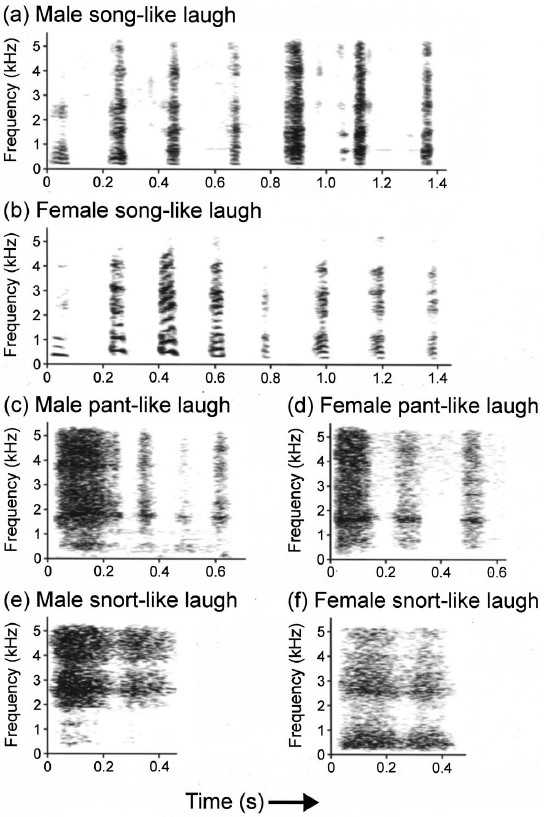
\includegraphics[scale = 0.62]{figs/laugh_spectrogram_from_bachorowski.png}
	\caption{Spectrogram visualisations of laughter from each of the tree different classifications in Bachorowski's paper. The difference in frequency structure of each laugh is easily seen, with harmonics in song-like laughter much more apparent.\cite{bachorowski2001acoustic}.}
	\label{laughter_spectrogram_from_bachorowski}
\end{figure}
% Different situations when laughter is different.
\noindent
Laughter also changes when produced under different circumstances. In N. Campbell's paper: ``Whom we laugh with affects how we laugh''\cite{campbell2007whom} a neural network is created and training on a single persons laughter when talking to a range of different people. The network learns to discriminate (with an accuracy slightly below 50\%) between with whom the speaker is speaking purely by the difference in laughs they make, proving that there is some difference in laughter features in different situations. This paper focussed on the differences in laughter when talking to people of different gender and of different ethnicity.\\
\\
% Biological laughter production
\subsubsection{Laughter Production}
% Laughter averages, ie frequency, length, call number, all that.
Laughter is a complex physical response, involving many different sections of the body. A number of studies look at the different bodily actions that occur during laughter. These responses can be seperated into five different areas:\cite{cosentino2016quantitative}
\begin{itemize}
\item Acoustics (The emitted sound)
\item Respiration
\item Phonation (The audio features, or shaping, of the emitted sound)
\item Facial Expression
\item Whole body movement
\end{itemize}
Recently a number of studies attempt to detect laughter by analysing a number of these different modes of expression simultaneously.\cite{petridis2008audiovisual,scherer2009multimodal} From an acoustical standpoint, laughter has several easily measurable features. These have been measured in many different studies, but averages for each of them have been found in a paper summarising hundreds of papers studying laughter written by S. Consentino\cite{cosentino2016quantitative}, and these are the numbers quoted below. A typical mirthful laugh contains four or five calls, and the average length of a call is about 220ms. Earlier calls tend to be louder than later ones, most likely due to a decreasing air supply. For both male and female laughter, the typical fundamental frequency is approximately 20\% higher pitch than in casual speech at ~278Hz for males, and ~480Hz for females. Voiced pulses may contain audio at a frequency higher than 16kHz, but most power is contained below 8kHz. The precise phonation of laughter has been measured precisely by using invasive intramuscular electromyogram signals.\footnote{These studies placed bands around the abdomen and chest of the patients and up to four small electrodes were injected into different laryngeal muscles. Despite having many electrodes embedded in their throats, the patients were all able to speak, swallow, and laugh comfortably.} Very complex analysis has been done on these detailed tests, revealing precisely how all the different muscles in the throat and neck move during laughter. Such descriptions are heavily biological, for example: ``During adduction, the thyroarytenoid and the cricothyroid muscles close the glottis, the arythenoids approach each other at a constant rate, and the vocal folds start vibrating while they are still not fully closed. Instead, during abduction, the posterior cricoarytenoid muscle is responsible for the opening, and the vocal folds are still vibrating when the abduction phase begins.''\cite{cosentino2016quantitative}\\
\\
While the precise movements of all the larynx and throat tissues isn't exactly required to develop a laughter detector, it is important to note the complexity of the structure of laughter, and the many different contributing factors which go into the creation of its sound. Analysis into the cause of differing laughter pitch alone is complex: ``Changes in the fundamental frequency F0 might be determined by multiple factors: the shortening of vocal tract length, due to lowering or lifting of the larynx, or to protraction or retraction of the lips, the tension and lengthening of vocal cords, and the variation of tracheal pressure which can, but not always, be temporally correlated with laryngeal adductors.''\cite{cosentino2016quantitative} It is this complexity to laughter which makes creating a laughter detector utilising purely phonetic theory such a hard task. Indeed, when talking about the different factors which make up laughter, Fry and Rader state: ``The interaction of these factors generates an almost infinite number of individually different laughs.''\cite{fry1977respiratory}

\subsubsection{The Social Role of Laughter}
% Laughter as it relates to social interaction.
% Social standings and heirachy.
Laughter is most often induced by something funny, and is a powerful conveyor of information. Laughter shows involvement in conversation and lets other people know that you have found something humerus. Besides this most common form of laughter, it can also be used to express other emotions such as stress and frustration. Another interesting observation is that people laugh more often when people around them are laughing. This is why laughter is often said to be `contagious'. This may be why the first comedian at a comedy club is tasked with `warming up the crowd', and laugh-tracks in sit-coms are employed to make a show seem more entertaining.\\
\\
% Simply as a sound
The interactions between laughter and speech are quite interesting. In a polite conversation between two people, most often only a single person is talking at one time and interruptions are kept to a minimum. Laughter is the opposite and if someone laughs, it is socially acceptable to laugh at the same time, and often politeness brings us to laugh when someone else does, even if we do not find anything particularly funny.\cite{dupont2014acoustic}\\
\\
% Power
As previously mentioned in subsection \ref{subsection:laughter}, laughter is used very differently depending on the social situation it is used in. One area of study in this field is the use of laughter in different power dynamics. In a paper by C. Rees, she looks in detail at a number of conversations which occur in a patient-doctor-student situation at a doctors office. In these scenarios there is a doctor and a student working directly under the doctor consulting a patient. The role of power in the workplace is looked at through the use of laughter by all parties. She concludes that: ``The laughables can be construed as teases of various kinds: fallibility, frustration, cynicism and/or sexual teasing. Although some of the teases may have been attempts by participants to construct intimacy, we believe that the teases functioned primarily to construct power, identity and gender.''\cite{rees2010should} In another paper looking at laughter in social work, it is noted that there is much more laughter between the social workers than there is between their clients. It is concluded that laugher is used: ``(Laughter is) employed by staff members as: (1) a way to create informal settings between staff and clients; (2) a way to deal with situational tensions/ambiguity in the work; and, (3) a way to deal with organizational contradictions in working with clients.''\cite{mik2007interpersonal}\\
\\
In a study by J. Bachorowski, students at a university listened to different recorded laughter segments for several people, and told to rate each subject in terms of `how interested to meet them' they would be. They found that both males and females are much more interested in meeting someone who uses voiced laughter more often than unvoiced grunts, pants, and snortlike sounds.\cite{bachorowski2001not}\\
\\
Highlighted by these studies is the large amount of depth for the different uses of laughter in social situations. This again draws attention to the large variety of different laughter types used in common situations, and the difficulty of laughter detection.

%\subsubsection{Health Perspective}
%% Laughter from a health perspective
%idk if this is even worth talking about given the small amount of research done here, and how hand-wavey it is.

% Laughter synthesis
\subsubsection{Laughter Synthesis}
Laughter synthesis has only been attempted recently, with computers becoming powerful enough to attempt to synthesize it. Since laughter is such a varying signal, it is particularly hard to recreate. Such laughter synthesis attempts focus solely on voiced laughter, rather than also attempting to recreate with `windy' sounds of unvoiced laughter. The ultimate goal of synthetic laughter generation is to create a realistic laugh, indistinguishable from a recording of real human laughter. As such, the most effective method of evaluating laughter `naturalness' is to survey a number of people about a number of laughter segments generated by each method and compare this to a control group of recorded human laughter. The most recent attempts at human laughter synthesis use hidden Markov models to generate a sequence of phonemes (most commonly the breathy `h', `a' vowel, and $\epsilon$ representing silence) which are then recreated using the STRAIGHT (Speech Transformation and Representation using Adaptive Interpolation of WeiGHTed spectrum) method.\cite{kawahara1999restructuring,dupont2014acoustic}
\begin{figure}[H]
	\centering
	\vspace{0.5cm}
	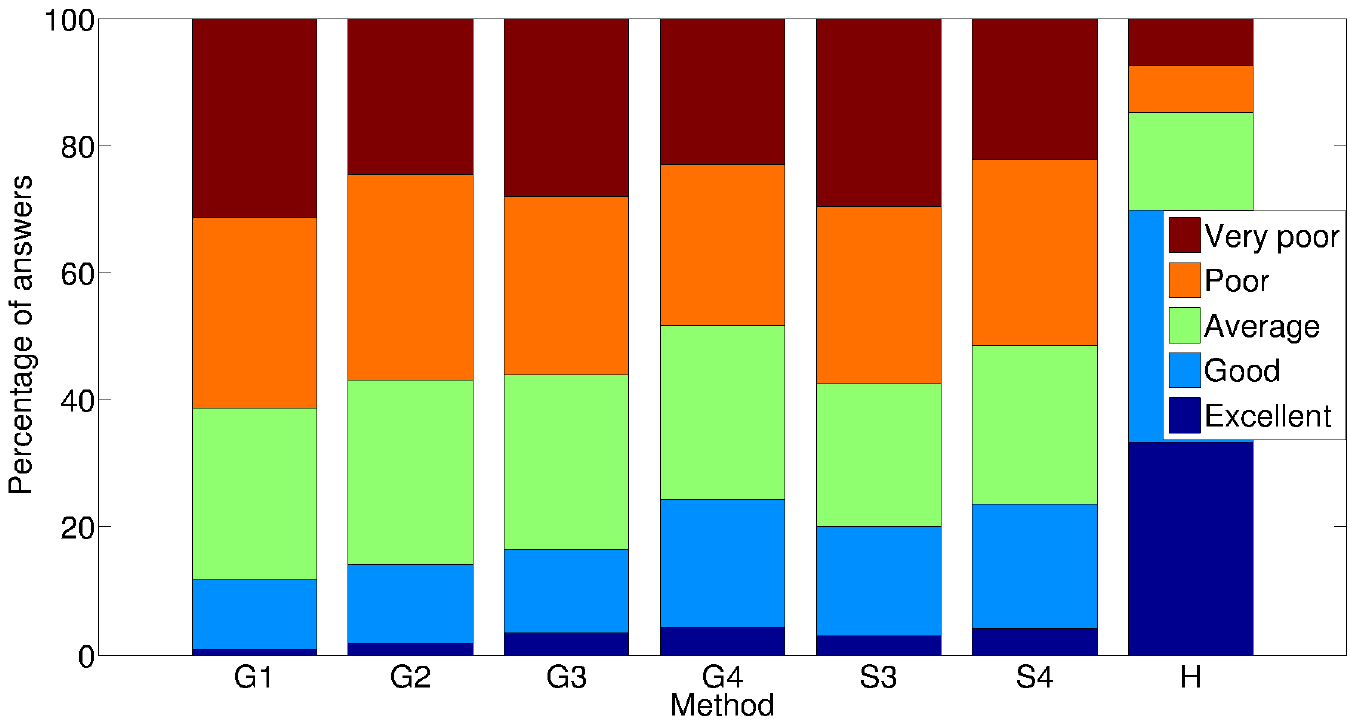
\includegraphics[scale = 0.35]{figs/laughter_naturalness.png}
	\caption{A plot of the naturalness of laughter created by J. Urbain's state-of-the-art laughter generator. The classes G1-G4 and S3-S4 are different laughter generation methods used in his study, compared to the H class which represents real human laughter. As can be seen from this image, laughter synthesis is still in its early days.}
	\label{laughter_synthesis_naturalness}
\end{figure}
Examples of synthesized laughter from each of the categories in Figure \ref{laughter_synthesis_naturalness} can be found at: \url{http://www.tcts.fpms.ac.be/~urbain/arousal_driven_synthesis/}.\cite{dupont2014acoustic}

\newpage

\subsection{Datasets}

% Talk about the datasets used in other papers, and how these differ from ours, and how the results will be impacted by this.
One of the most important aspects of any machine learning problem is the procurement of a good quality dataset to train a model on. Several databases with pre-labelled laughter exist, and this section aims to analyse these databases in terms of their effectiveness in training a laughter classifier.\\
\\
In his PhD thesis on laughter synthesis\cite{dupont2014acoustic}, J. Urbain does an extensive analysis of different existing corpora of speech and laughter. I have summarized his findings into table form in Table \ref{table:table_of_databases}. The table highlights the most important factors when choosing a dataset:
\begin{itemize}
\item The stimulus of the laughter.
\item The size of the corpus, in time or laugh count.
\item How the laughter is classified.
\item The availability of the dataset.
\item The form of the data in that particular corpus.
\end{itemize}
The stimulus of the laughter in each corpus is very important, because as shown several times in Section \ref{subsection:laughter}, the type of laughter produced is heavily dependant on the situation the subject is in. I have given the label `Spontaneous' to any dataset featuring laughter which has arisen naturally. For example, any unscripted or casual conversation would feature spontaneous laughter. There are also datasets where subjects were asked to laugh (classified as `Scripted') or made to watch funny videos in order to create laughter (classified as `Induced'). It may also be important to note that in the MANHOB dataset, lab personnel remained in the room with the subject, which would almost certainly effect the recorded data, as it has been shown that humans alter there laughter depending on their company.\cite{campbell2007whom} It is estimated that the presence of researchers would increase the amount of nervous laughter in the recordings. If this dataset was used to train a laughter classifier, it would potentially bias the system towards nervous laughter, and not spontaneous laughter.\\
\\
The number of laughs in the corpus is equally important. In machine learning problems, more data is always better as it allows larger generalization and a higher accuracy. Some corpora contain very few laughs, on the order of < 100, while other contain many thousand.\\
\\
The classification style of the laughter is also paramount. In order to train a classifier on laughter, the exact start and stop times of the laughter must be known. However, most corpora either flag positions of laughter, or simply transcribe it in text. This helps, because it would make selecting laughter easier in that the whole text doesn't need to be listened too, and the sections containing laughter could be jumped to directly to more accurately classify.\\
\\
The availability of the corpus is also noted. The best dataset in the world is of little use to anyone if it is not accessible. This thesis study has a small budget of < \%500 AUD, which rules out many more expensive datasets by default.\\
\\
And lastly the type of data contained within the dataset was noted. Some datasets contain only audio, while other multi-modal datasets contain recordings from a variety of media, from fully body and facial video, to 3D body modelling, and thermal imaging.
\begin{landscape}
\renewcommand\arraystretch{1.5}
\begin{longtable}{|p{3cm}|p{4cm}|p{2cm}|p{3cm}|p{3.5cm}|p{3cm}|}
\hline
\textbf{Name} & \textbf{Stimulus} & \textbf{Size} & \textbf{Laughter Classification} & \textbf{Availability} & \textbf{Data Type} \\ \hline \hline
Corpus of Spontaneous Japanese & Spontaneous (Recordings of lectures and presentations) & 650 hours of speech & Labels, no time boundaries & \$280 AUD for academics, \$2800 AUD for commercial use. & Audio \\ \hline

FreeTalk Database {[}Campbell 2007{]} & Spontaneous (Telephone conversations) & 20 hours & Time aligned phonemes. Transcription. & Free for academics. Must apply with university email and be individually accepted. & Audio \\ \hline

Santa Barbara Corpus of Spoken American English & Spontaneous (Casual conversation) & 249,000 spoken words & Transcriptions & Free Online & Audio \\ \hline

The Corpus Gesproken Nederlands (CGN) & Spontaneous / Scripted (Recordings of numerous situations. News reports, lectures, casual conversation) & 550 hours / 650,000 words. & Non-speech events tagged. & \$2,600 AUD for Academic Research - \$22600 AUD for Commercial & Audio \\ \hline

COSINE Database & Spontaneous (Casual conversation) & 10 hours transcribed. & Laughter events marked. & Free & Audio \\ \hline

ICSI Meeting Corpus & Spontaneous (Recordings of meetings) & 85 hours & Laughter events start and end times marked. & \$2400 AUD & Audio / One microphone per person \\ \hline

The MMLI Corpus & Spontaneous (games with friends) & - & Laughter events annotated. & Free for academics, though not easily available. & Audio, facial and full body video, inertial motion capture. \\ \hline

MMI Facial Expression Database & Induced (Watching video clips) & 164 laughter instances & Transcribed & Free for academics, through not easily available. & Audio, Video \\ \hline

Belfast Induces Natural Emotion Database & Induced (Watching video clips) & 289 laughs & Laughter has been extracted and saved separately. & Free for academics. & Audio, Video \\ \hline

MANHOB Laughter Database & Induced / Scripted / Very artificial environment. & 563 laughs / 931s laughter duration & Laughter segments fully classified with ELAN. & Free & Audio, Video, Thermal Video \\ \hline

Green Persuasive Database & Spontaneous (During conversation) & 280 laughter instances & - & Free for academics, thought not easily available. & Audio, Video \\ \hline

SEMAINE Database & Induced (Watching video of automated avatar) & 5.5 hours of audio. & Emotional States have been labelled. Not laughter. & Free for academics. & Audio, Video \\ \hline

\caption{Table of speech and laughter databases.}
\label{table:table_of_databases}
\end{longtable}
\end{landscape}
% Further discussion about the ICSI database
\subsubsection{ICSI Database}
The most commonly used database in this table is the ICSI Meeting corpus, and it deserves a little extra discussion. This project began in 2000, and collected 72 hours of speech from meetings that ``would have occurred anyway''\cite{janin2003icsi}. Each of the several participants in the meeting were given head mounted microphones and recorded individually, as well as one other microphone left in the table between them to record all audio. Highly detailed transcriptions of these recordings were created, where the start and end time of every utterance is marked. Many different non-speech sounds were also marked, such as laughter. The frequency of each of these non-vocal sounds is shown in Table \ref{table:icsi_meeting_utterance_frequency}\cite{laskowski2007correlation}. While the ICSI database was not created to investigate laughter, due to it's large number of precisely labelled laughs, several papers analysing the frequency and use of laughter within these meetings were written. Also, this dataset is the most used dataset in laughter detection, with several papers all using these transcriptions to develop laughter classifiers.\cite{kennedy2004laughter,truong2005automatic,knox2007automatic} These papers mostly used the original labelling of the laughter, and occasionally modified it to exclude `bad' laughter segments (Segments which contained faint of near inaudible laughter, or overlapping speech and laughter)\cite{truong2005automatic}.

\begin{table}[H]
\centering
\begin{tabular}{|l|l|l|}
\hline
\textbf{Frequency Rank} & \textbf{Token Count} & \textbf{VocalSound Description} \\ \hline \hline
1                       & 11515                & laugh                           \\ \hline
5                       & 970                  & breath-laugh                    \\ \hline
11                      & 97                   & laugh-breath                    \\ \hline
46                      & 6                    & cough-laugh                     \\ \hline
63                      & 3                    & laugh, "hmmph"                  \\ \hline
69                      & 3                    & breath while smiling            \\ \hline
75                      & 2                    & very long laugh                 \\ \hline
\end{tabular}
\caption{A table showing the frequency of laughter related non-speech utterances in the ICSI meetings database\cite{laskowski2007correlation}.}
\label{table:icsi_meeting_utterance_frequency}
\end{table}

\noindent
The ICSI would have been near perfect for this thesis if it were more accessible. The cost to obtain this dataset is \$2400 AUD, which rules it out as an option for this study.
% Further discussion about the MANHOB database
\subsubsection{MANHOB Database}
A second database which comes close to the quality of the ICSI database is the MANHOB Laughter Database. This database was specifically created for the study of laughter, and contains 563 instances of laughter. All audio has been annotated with ELAN\cite{sloetjes2008annotation}, so the start and stop times of each laughter segment are marked, and can easily be read out of ELAN's XML format for processing. Above all, this dataset is free to access and download for academics. However this database contains laughter stimulated by humorous videos while two operators are observing the subject in the same room. It also contains acted laughter. The presence of humans is known to change the types of laughs emitted \cite{campbell2007whom}, so this dataset can not be classified as `spontaneous'.\\
\\
% Conclusion paragraph
Although both the ICSI meetings database, and the MANHOB laughter database are excellent candidates for use, the cost of the ICSI database rules it out, and the small size and acted laughter of the MANHOB database rules it out too. It is because of these reasons that a new database was created for use in this study.

\subsection{Preprocessing}

% There is definately much more you can write on MFCC's here.
	% Comparison to PLP's
	% How exactly do MFCC's work?
		% Plus pictures.
	% Frame size and stride.
		% Plus picture.
	% Delta's and delta deltas

From the book: ``Fundamentals of Speech Recognition'', it is said that: ``... perhaps the greatest common denominator of all recognition systems is the signal-processing front end, which converts the speech waveform to some type of parametric representation (generally as a considerable lower information rate) for further analysis and processing.''\cite{rabiner1993fundamentals} The book goes on to dedicate an entire chapter to discussing and comparing the various different methods of signal processing used to extract series of features for the data input to a speech recognition system. As alluded to in that quote, this is especially important as it reduces the rate of information needed to be processed by the neural network. In another publication by world leading researchers: ``This non-adaptive but highly engineered preprocessing of the waveform is designed to discard the large amount of information in waveforms that is considered to be irrelevant for discrimination and to express the remaining information in a form that facilitates discrimination...''.\cite{hinton2012deep} For example: over a single second of audio, lets assume that a handful of syllables are pronounced by the speaker. All information in the time series waveform is not necessarily needed to understand which syllables were said. Rather than the 44000 floats used to describe the waveform over one second, signal processing techniques can be used to extract the amounts of different frequency sounds from the audio. This 44000 floats/second waveform can be reduced to roughly 1000 floats/second of extracted features. This is greater than an order of magnitude size reduction, while only losing a fraction of the audio information. This allows researchers to train networks on much larger datasets, for much longer than would be possible if the entire waveform were to be used.\\
\\
Feature extraction is the process of trying to retrieve meaningful features from our audio signal. Just by observing the vector of samples shown in Figure \ref{time-series}, or its spectrogram in Figure \ref{spectrum}, the general sound of the file can not be easily observed. A plethora of signal processing methods are implemented in an attempt to pull meaningful information out of the audio signal. Types of features can be broken down into two sections: frame-level features, and utterance-level features. The first is a set of features formed by analysing `frames' of audio usually about 20ms in length, and the latter contains information about the volume, pitch, and AC power of the surrounding $\sim$2 seconds of audio.\cite{truong2007automatic} Figure \ref{frames} shows a diagram of where these zones are calculated.
\begin{figure}[H]\vspace{0.3cm}
	\centering
	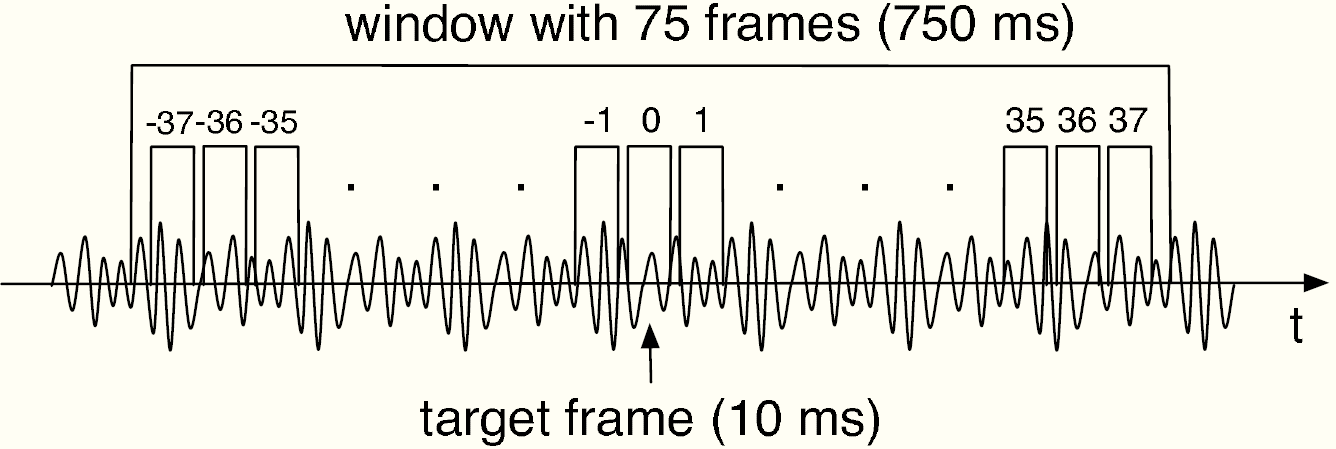
\includegraphics[scale = 0.40]{figs/frames}
	\caption{This image is a window spanning 75 smaller frames. Frame level features are calculated for each frame, but the utterance-level features are calculated for the whole window and calculated for each frame. This way, each frame holds valuable information about itself, and the 350ms on either side of it.\cite{knox2007automatic}}
	\label{frames}
\end{figure}

\subsubsection{Frame-Level Features}

Laughter detection uses many of the same popular features as speech recognition techniques. Some of the most common and successful techniques for extracting relevant features from frames of audio include using Mel Scale Cepstral Coefficients (MFCC’s)\cite{knox2007automatic,truong2005automatic}, Perceptual Linear Predictive (PLP) Coefficients\cite{hermansky1990perceptual}, MFCC deltas, and Mel Scale Filter Bank Energies (FBANK)\cite{gosztolya2016laughter}.\\
\\
Before looking at each type of feature available to use, it is worth considering the frame sizes used to extract these features. Figure \ref{frames} simulates an audio waveform, divided up into different sized frames, and a larger containing window. In this Figure, the frames are each 10ms long. Larger frames will capture more information by allowing for a more accurate frequency analysis of each frame, while smaller frames allow quick changes in frequency to be captured. For the best of both worlds, larger frames can be used, with consecutive frames overlapping. In this case, the `stride' is the amount of time between the start of two consecutive frames. If the frame size if 20ms, and the stride is 10ms, each frame will share 10ms with it's previous frame, and 10ms with the next frame. The frame size is a subtle change, but nonetheless it is a good idea to look to previous literature in order to find reasonable values. Frame sizes of 10ms\cite{kwon2003emotion}, to 25ms with a 10ms stride\cite{knox2007automatic}, and 32ms with a stride of 16ms\cite{truong2007automatic} are all used in laughter detection, so values around here are a good place to start.
\begin{figure}[H]
	\centering
	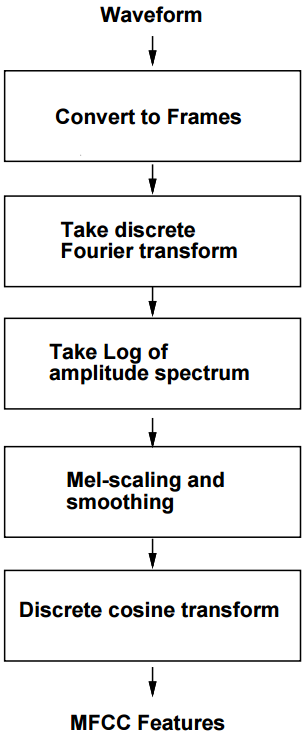
\includegraphics[scale = 0.6]{figs/mfcc}
	\caption{The steps taken to obtain the MFCC values.\cite{logan2000mel}}
	\label{mfcc}
\end{figure}
The goal of MFCCs and PLP values is to reduce the 880 values\footnote{This is assuming a 44Khz signal.} within 20ms of audio to $\sim$13-20 values which contain most of the important information of the audio signal. This lets computation be orders of magnitude more efficient, while only losing a small amount of the auditory data held in a snippet of audio. The steps to obtain the MFCC's are shown in Figure \ref{mfcc}. Examples of audio transformed to find MFCCs and transformed back again in an attempt to recreate the audio show that a large amount of the important features of the audio are retained in these 13 dimensions.\cite{Ellis05-rastamat}\\
\\
% Talk more about MFCC's here because we are using them in this report
MFCCs attempt to extract data from the audio time series in the way it is perceived by humans. As shown in Figure \ref{mfcc}, calculating the MFCCs takes the log of the amplitude of the audio signal because humans perceive volume at a log scale, while using the Mel Scale for frequency, which are frequencies of perceived equal pitch variation. MFCC-like techniques were first used to analyse the spectrum of vowel pronunciation and have always existed as a method of analysing speech.\\
\\
% Paragraph about exactly how to find them
MFCCs are calculated by first taking the Fourier Transform of the audio frame to extract the frequencies within the signal, then mapping these frequencies into the Mel Spectrum using a series of overlapping triangle filters. The log of the amplitudes is taken, and then the discrete cosine transform is taken of these mel-log powers. The MFCCs are the resulting features. Libraries to compute them can be found online\cite{Ellis05-rastamat}.\\
\\
% Talk about PLP's here
PLP coefficients attempt to find a set of values representing human speech in a similar way, but repress speaker-independent information. In the field of speech detection, PLP values are often slightly more accurate than MFCCs.\cite{psutka2001comparison} In the field of laughter detection, both MFCCs\cite{knox2007automatic,gosztolya2016laughter,kennedy2004laughter} and PLPs \cite{gosztolya2016laughter,truong2007automatic,truong2005automatic} have been used successfully, with very little variance in results for studies which have analysed both.\cite{gosztolya2016laughter}\\
\\
In addition to MFCCs and PLP coefficients, their deltas and delta-deltas also prove useful as features.\cite{knox2007automatic}. These features take into account the trajectory of the MFCCs or PLPs over time. Essentially the delta features are the time derivative of the original values, and the delta-delta is the double derivative. Since: ``Almost all current automatic speech recognition (ASR) systems conventionally append delta and double-delta cepstral features to static cepstral features.'',\cite{kumar2011delta} this is also a reasonable feature to include in laughter recognition, and has performed well in the past.\cite{knox2007automatic}

\subsubsection{Utterance-Level Features}

Utterance-level features of audio are features which take place over the course of approximately one second. Laughter has a repetitive nature, and so AC peak power over this time is a frequently measured value. Other features include the local RMS value, and the fundamental frequency of the segment. Using neural networks to analyse a system with these three features, the AC peak was determined to be the most useful in determining whether audio contains laughter, as it reduces error by $\sim$1.5\% when combined with MFCCs.\cite{knox2007automatic}

\newpage

\subsection{Laughter Discrimination Methods}

% Machine learning overview
After preprocessing the audio signal, a list of features for each frame is left. Various methods and statistical models can be employed to learn from these data points and laughter and speech in audio. Methods used in the past for these objectives will be analysed in the sections below. The different methods to detecting laugher can be broken down into two different areas: statistical models, and machine learning. Statistical models include algorithms such as Support Vector Machines (SVMs), Gaussian Mixture Models (GMMs) and Hidden Markov Models (HMMs), while machine learning is a much newer field where computers attempt to detect higher level features from data without them being explicit programmed into the model.

\subsubsection{Statistical Models}

% Statistical models
	% Markov models, and all other models used in previous papers.
After processing the audio into its features, there are several different ways to attempt to classify it into simply `laughter' and `not-laughter'. SVMs, GMMs, and HMMs all begin by treating each frame as a point in $n$ dimensional space, where $n$ is the number of features there are in the frame. So if we are using the first 10 MFCCs, then we plot every frame as a point in 10-dimensional space. At this point these three methods deviate.\\
\\
In a support vector machine, a plane is drawn through the n-dimensional space to attempt to discriminate between different clusters. For example, if frames containing laughter are different to all other frames, then you would expect to be able to discriminate them easily from all other sounds, as they will all be positioned uniquely in n-dimensional space. By using a kernel function, this discriminating plane can be curved to give the most accurate separation. This method was used in the first published attempt at laughter detection.\cite{kennedy2004laughter}\\
\\
Gaussian mixture models take a different approach. After placing all the points in n-dimensional space, it creates a number of Gaussian distributions, and iteratively tweaks the covariance matrix of the Gaussion distribution to more closely fit the distribution of the frame samples. This method also assumes that frames of laughter are different to frames of non-laughter, and should be able to be discriminated because they lie in a different location in n-dimensional space. This method has been used to attempt to classify laughter in the past.\cite{truong2005automatic}\\
\\
Hidden Markov models are slightly different, but begin like a Gaussian mixture model. After placing all the frames into the n-dimensional space, a Gaussian mixure model is used to create groupings of similar frames. Next, it is assumed that there are some hidden states of the system. For example: laughter and not-laughter. Each of these states has a probability of producing outputs in each of the Gaussian distributions of points. By observing the sequences of frames, the hidden state of the system can be estimated by using Bayesian inference. This method has found applications in the fields of speech tagging, speech and laughter synthesis\cite{dupont2014acoustic}, and speech recognition. It has also been used to detect `paralinguistic events' in audio such as laughter and applause.\cite{cai2003highlight}

\subsubsection{Machine Learning}

Machine learning is a term coined for the creation of programs to help computers learn high-level tasks, without being explicitly programmed to do so. In recent years, these networks have found great successes in the fields of image classification\cite{ciregan2012multi}, language translation\cite{bahdanau2014neural}, and speech recognition\cite{graves2013speech} to name a few. Neural networks are algorithms which take inspiration from a basic model of how neurons in the brain work. As seen in Figure \ref{artificial_neuron}, a number of inputs enter the system, are multiplied by a number of weights, added together, and multiplied by an activation function. If the sum is sufficiently high, the neuron will activate, otherwise it may not. This output is either used as the output of the system, or an input into another neuron. By creating systems with many layers of hundreds of neurons, high level features can be determined.\\
\\
Neural networks must be `trained' before they can classify data. The process of training involves calculating the outputs of the network for an input with an already known output. After each set of inputs is shown, the weights are changed a little to make the output closer to the known output through a process known as `back propagation'. After many thousands of weight updates in the training phase, when the system is shown a set of inputs it should be able to correctly classify the output. The goal is to learn a general rule pertaining , the outputs should represent the class that the inputs belong to.\\
\\
This basic type of neural network is called a feed-forward neural network. Both single, and multi-layer feed-forward networks have been used to detect laughter in audio.\cite{knox2007automatic,gosztolya2016laughter}

	% Neural networks

\begin{figure}[H]
	\centering
	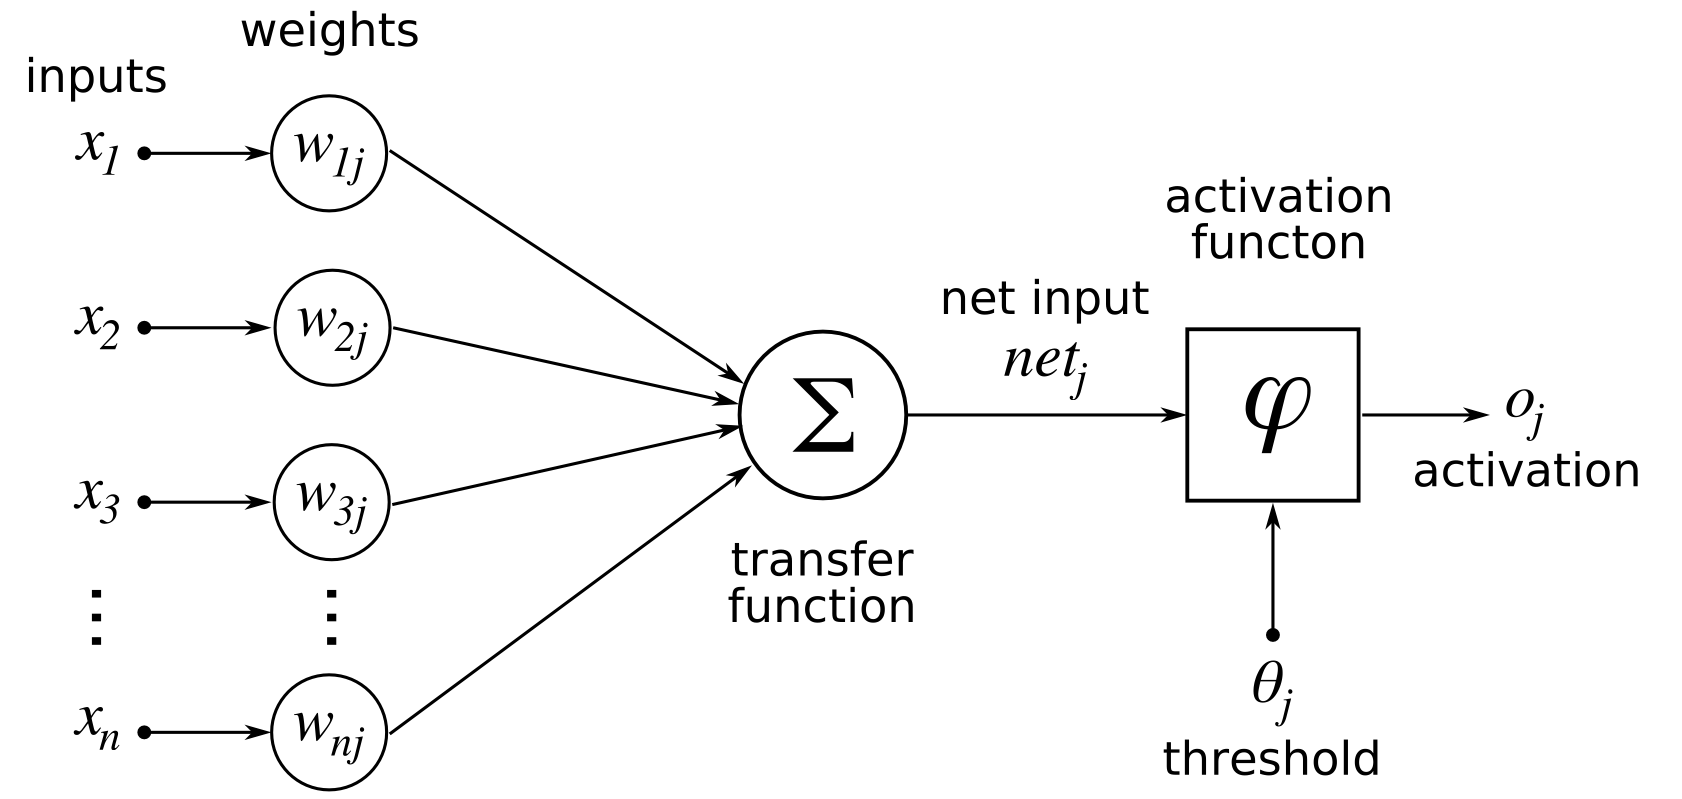
\includegraphics[scale = 0.2]{figs/artificial_neuron.png}
	\caption{A model of an individual neuron in a neural network.}
	\label{artificial_neuron}
\end{figure}

	% lstm networks
\noindent
Recurrent Neural Networks (RNNs) and Long Short Term Memory units (LSTMs) are different neural network models specifically designed to classify temporal signals. Recurrent neural networks have layers which feed back into themselves and/or previous layers, giving the system information about previous inputs. Recurrent neural networks encounter a problem known as the `vanishing gradient problem', in which older inputs contribute less to the output of the network. LSTM units were created to solve this, and can retain information about features mentioned in the past to influence the current outputs. LSTMs have improved speech to text\cite{graves2013speech}, recognition of context sensitive languages, and handwriting recognition\cite{greff2016lstm}.

\newpage

\subsection{Previous Laughter Detection Attempts}

% In this section we will talk about other laughter detection papers.
% Definately discuss the metrics they use to talk about accuracy at some point.

There are several papers which have attempted to detect laughter in the past. One of the first is a paper by R. Cai\cite{cai2003highlight}, which uses a hidden Markov model to detect laughter amongst other audio features in a set of videos. To process the audio, it was split up into one second chunks, and MFCCs amongst other features were used to classify these chunks. They achieved error rates from 12\% to 22\% depending on the video. Unfortunately, this study used only three videos, for a total of two hours of audio. This is not really sufficient enough to learn the general structure of laughter, but this first study shows that it is possible to obtain better than random laughter detection.\\
\\
Another paper by L. Kennedy and D. Ellis\cite{kennedy2004laughter} attempts to classify laughter from non-laughter using a SVM trained with a number of features from the ICSI database, including MFCCs. The audio was segmented into one second samples, and a sample was classified as laugher if larger than a certain amount of that sample contained laughter. Their most accurate prediction has an equal error rate of 13\%. Two main conclusions from this paper are that:
\begin{itemize}
\item MFCCs one through six are the most important features to use in laughter detection. Kennedy and Ellis trained systems with a number of different features to test results, and the performance of these results is shown in Figure \ref{icsi_performance_features}. Using MFCCs as features perform more accurately than any other method, and the authors note that including the other features with the MFCCs doesn't meaningfully increase the accuracy of the results.
\item Using the ICSI database as a training set, and testing on audio from other databases can have very mixed results. On certain datasets, laughter detection rates little more than random guessing were recorded.
\end{itemize}
\begin{figure}[H]
	\centering
	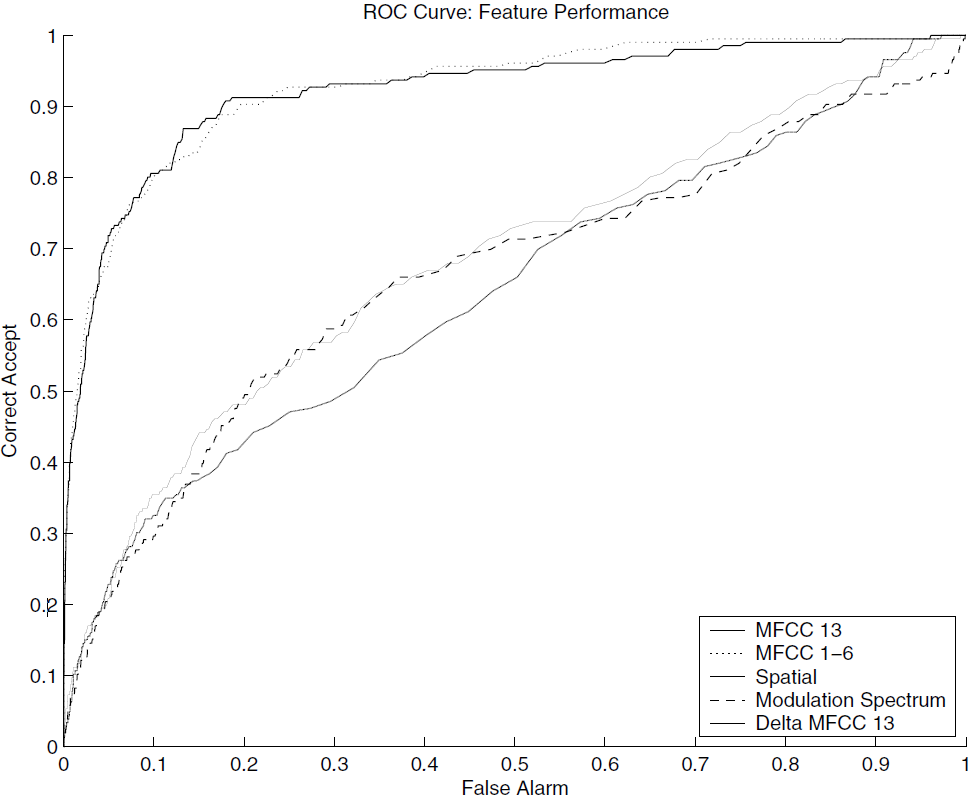
\includegraphics[scale = 0.4]{figs/icsi_performance_features.png}
	\caption{Performance of a trained SVM on the test set of laughter, using different sets of features. It can be seen that the two sets of features: ``MFCCs 1-6, and MFCCs 1-13'' perform roughly equally, and much more accurately than any other sets of features.}
	\label{icsi_performance_features}
\end{figure}
Building on this initial work is another paper by K. Truong and D. van Leeuwen\cite{truong2007automatic}. They use Gaussian mixture models to train a classifier on the ICSI database, yielding a minimum equal error rate of 15.6\%. When using the same classifier on laughter from the Dutch CGN corpus, the error rate dropped to 20\%. Truong and van Leeuwen showed that using PLPs as features for laughter detection yield results on par with that from MFCCs. They mention in their conclusion: ``Another suggestion for future research is to develop a laughter detection model that is also able to determine the beginning and end of laughter. So far, we have used presegmented data to detect laughter. A laughter detection model that also provides an automatic time alignment of laughter is a more complex task that gives rise to additional problems such as: how do we decide when a laughter starts or ends and how do we evaluate the performance of such a detection model?''\cite{truong2007automatic} This is what this paper attempts to solve.\\
\\
Later in the same year M. Knox and N. Mirghafori attempted to recognise laughter using neural networks for the first time\cite{knox2007automatic}. They recorded a minimum equal error rate of 7.9\% on the ICSI meeting database, using the same test set and training set as K. Truong in their paper\cite{truong2007automatic}. The model found to be most accurate by Knox and Mirghafori used a `context window' of 75 10ms frames of audio for which features were calculated. The most accurate system used 12 MFCCs and the AC peak of each frame. Their network had a single hidden layer of 200 nodes.\\
\\
All previously discussed papers use only audio to detect laughter. There are a number of papers focussing on using multimodal databases, and classifiers which use audio and visual features to detect laughter. B. Reuderink\cite{petridis2008fusion,reuderink2008decision} used the AMI meeting corpus to find and classify chunks of audio which may or may not contain laughter. This study only trained on 40 laughter instances however, so it is not expected that any very high level features will be learnt.\cite{petridis2008audiovisual} Alongside the standard MFCC feature collection most papers use, Reuderink also tracks 20 points on the faces of his subjects. The cartesian $x$ and $y$ positions of these points are concatenated to give a 40 dimensional vector, of which the 12 most signifigant vectors are extracted from using Principle Component Analysis (PCA). The best results on this dataset achieve a 14\% equal error rate. Another study on multi-modal laughter detection draws bounding boxes around the faces of subjects using the Viola Jones approach and the movement on these faces was used as the visual data along with MFCCs for the audio.\cite{scherer2009multimodal} This method yielded an accuracy\footnote{The paper never mentions exactly what type of accuracy they are talking about here.} of 90.5\%.\\
\\
Most recently, a group of Hungarian researchers attempted laughter classification using deep rectifier neural networks\cite{gosztolya2016laughter}. They used two different datasets: the BEA Hungarian Spoken Language Database, which contained 332 laughter segments, and SSPNet Vocalization Corpus which is English and contains 2988 laughter segments. G. Gosztolya managed to achieve errors between 0\% and ~15\% depending on the database.\footnote{The Hungarian database consistently performed much better than the English dataset in this paper.} The network employed to obtain such results contains three hidden layers of 256 rectifier neurons each.

\newpage

\section{Methodology}

% How I've gone about my work. So this is the major heading talking about what I've done to attempt to detect laughter.
% I am unsure about whether to actually put any writing about anything in this section, or just put it all into the subsections.

When this project was started, there was no dataset or prior work on this topic, so everything from dataset procuring to network design was created for this project. This section details all the steps that were taken for each fundamental part of this project.

\subsection{Dataset}

% Starting with all my working into the dataset.
	% Talk about the audio of the dataset first.
		% How it was recorded
		% When
		% What it was for
		% The type and quality of audio
		% General statistics about the laughter.
		% Compare my dataset to other datasets and talk about the differences.
	% Preprocessing of the dataset. Removing noise. Normalizing volume roughly.
	% Talk about classification of laughter
		% My classification.
		% Compared to other peoples classification and maybe error analysis.

For the type of laughter detector being created, a large amount of audio with signposted laughter start and stop times is required. The best, spontaneous speech dataset containing laughter classified as required is the ICSI database. This has been used in several other studies attempting the classification of laughter, and would allow our system to be compared directly to other researchers. However, the high cost of obtaining this dataset does not allow it to be used for this thesis. Instead a new laughter database was created from audio from the Australian National Corpus \cite{johnston2009creating}.\\
\\
The dataset used for this project was a collection of recorded spontaneous speech from the Australian National Corpus. A total of eighty-one different audio clips were used, for a total audio length of fifteen hours and twenty-six minutes. These audio snippets contained conversations from students in the school yard, interview type scenarios, casual around-the-house conversation, and a variety of people in different scenarios. A majority of the recordings were taken over twenty years ago on cassette tape, and have been since converted to digital format. Conversations most frequently occur between two or sometimes three people, with the occasional recording containing more. This is important to note, as this thesis details the detection of laughter by one person, and not the detection of laughter of many people at once, as is done in other papers \cite{kennedy2004laughter}, and therefore occurrence of laughter from multiple people may cause issues for classification.\\
\\
The recordings used from the Australian National Corpus have been recorded using a variety of equipment, in a variety of different situations. The different audio files contain background noise from many different sources. Past research has found that laughter detectors have a much higher accuracy when testing audio recorded in the same way as the training data [REFERENCE], and potentially this variety in our dataset may increase the accuracy laughter detection for audio from other datasets. On the other hand, it may increase the difficulty of learning the form of `laughter' and increase the difficulty of classifying laughter.\\
\\
This corpus is smaller than the datasets used in other studies, which have used hundreds of hours of audio from recorded meetings, or telephone calls. It is well known that machine learning techniques improve where there is more data, and with only fifteen hours of audio, our results will be limited. The laughter in the audio used in this study is very diverse, with many different types of laughs. There are long belly laughs from old friends, and very short polite laughs from a child addressing their parents. There are laughs from people with thick accents, and laughs emitted which trying to talk. The diversity of the dataset used is an advantage, as any patterns learnt should be to the nature of laughter 'in-general' and not overgeneralise to a specific type of laughter, or the laughter of one person.\\
\\
All audio files are purely recordings of human speech, and do not contain noises from other sources, allowing the classifier to discriminate between human speech and laughter. Perhaps including sounds from other objects (random sounds, ie: trains, popping bubbles, waterfalls) in the training set could increase the robustness of the classifier.

\subsubsection{Classification}

Prior to this study, the audio from the Australian National Corpus had never been used for laughter detection, and the data labels did not exist. Past research has labelled audio in many different ways for laughter detection. Sections of audio containing laughter have been flagged, individual instances of laughter have been flagged, or most accurately, the laughter start and stop times have been individually labelled. The most recent work on laughter detection using the ICSI meeting corpus uses the start and stop times of `laughter' annotations which are seen in Table \ref{icsi_performance_features}. In these studies, researchers used these annotations, and slightly modified them when the data labels were found to be inaccurate \cite{knox2007automatic}. However, with hundreds of hours of audio, sifting through it all manually to select the laughter would be infeasible. In this study, the audio files from the Australian Nation Corpus were listened to, and the laughter segments were manually selected down to the millisecond.\\
\\
The method used to classify the laughter, was to use ELAN\footnote{ELAN is a product of the Max Planck Institute for Psycholinguistics, The Language Archive, Nijmegen, The Netherlands. It is free, and can be found here: \url{http://tla.mpi.nl/tools/tla-tools/elan/}}\cite{sloetjes2008annotation}, an audio-visual transcription software, to select the sections of audio which contain laughter. ELAN outputs this data in an XML format, which is parsed into a list of times when laughter starts, and then subsequently stops. These lists of start and stop times are used when creating the dataset, and the label (in one-hot encoded form) is appended to the vector of audio features. This list of start and stop times can also be quickly analysed to give some insight into the frequency and average laughter length in the collected dataset. The average laughter time of roughly one second in Table \ref{laughter_stats_table} agrees with findings from previous studies about the nature of laughter.\cite{bachorowski2001acoustic}\\
\\ 
\begin{table}[]
\centering
\begin{tabular}{|l|l|}
\hline
Total Laugh Count                     & 1456           \\ \hline
Total Length of Laughter              & 1480.1 seconds \\ \hline
Longest Laugh                         & 6.32 seconds   \\ \hline
Average Laugh Length                  & 1.01 seconds   \\ \hline
Audio File with Least Laughs Contains & 0 laughs       \\ \hline
Audio File with Most Laughs Contains  & 102 laughs     \\ \hline
\end{tabular}
\caption{A table containing statistics of the laughter classified in the complete dataset.}
\label{laughter_stats_table}
\end{table}

\begin{figure}[H]
	\centering
	\vspace{0.5cm}
	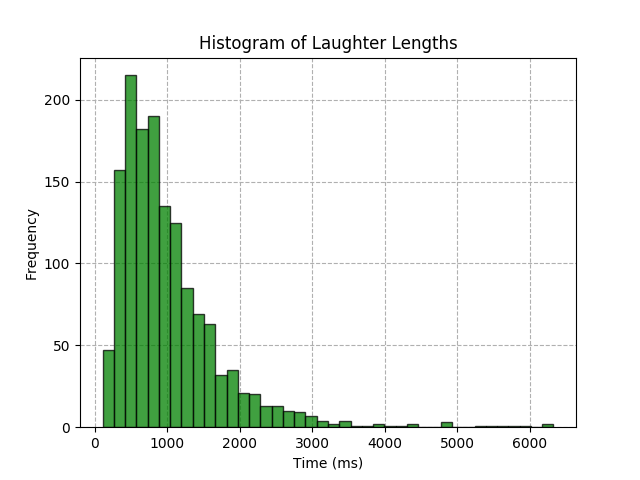
\includegraphics[scale = 0.8]{figs/laughter_length_histogram.png}
	\caption{A histogram of the laughter segment lengths.}
	\label{laughter_length_histogram}
\end{figure}

\noindent
Laughter in speech is a hard audio signal to classify. It often does not have a definite start or end point. Commonly an individual laugh will be preceded by a sharp inhalation, and/or followed by a brief `ahh' sound, and every laugh is different. Some might be very quiet snickers, snorts, or just fast exhalations. What do we empirically classify as `laughter'? Rather than define `laughter' as a specific type of laughter, potentially an easily distinguishable laughter like a belly-laugh, which would make the job of classification much easier, the data was classified as what the author `felt' was laughter. In order to train a model to predict laughter as accurately as a human, it needs a human-like classification. This makes this section particularly tough to write as scientists don't enjoy saying: ``This particular section of audio `felt' like laughter'', but would rather employ some quantitative analysis to say: ''This audio is definitely laughter because...''. When it comes to machine learning with audio, we want to give the model something a human thinks is correct, and let the machine find the complex mathematical relationships which separate laughter from non-laughter. This means that while previous papers have, for example, not classified the exhalation after the laugh as laughter\cite{bachorowski2001acoustic}, this report may have, so slightly different finding with respect to laughter lengths are expected.\\
\\
Nevertheless, when classifying laughter, what one person `feels' is laughter, is almost certain to not be identical to the observations of another person, and this is worth investigating. In an effort to investigate differences in laughter classification between different people, and determine the accuracy of the laughter detection of the author, two people were taught how to classify laughter using ELAN, and given a 45 minute audio clip to classify.\\
\\
In this 45 minute clip, one classifier found 87 laughter instances, and the other found 61. The actual classifications were very similar however. The main differences are that one classifier often split longer laughter segments up into multiple pieces, and included segments of laughter interwoven with speech. Example plots of the difference classifications are shown in Figure \ref{laughter_classification_differences_1} and Figure \ref{laughter_classification_differences_2}. With more classifiers, the jerky transition between laughter and non-laughter will be smoothed. Even without more classifiers, a linear interpolation method could be employed to further smooth these transitions.
\begin{figure}[H]
	\centering
	\vspace{0.5cm}
	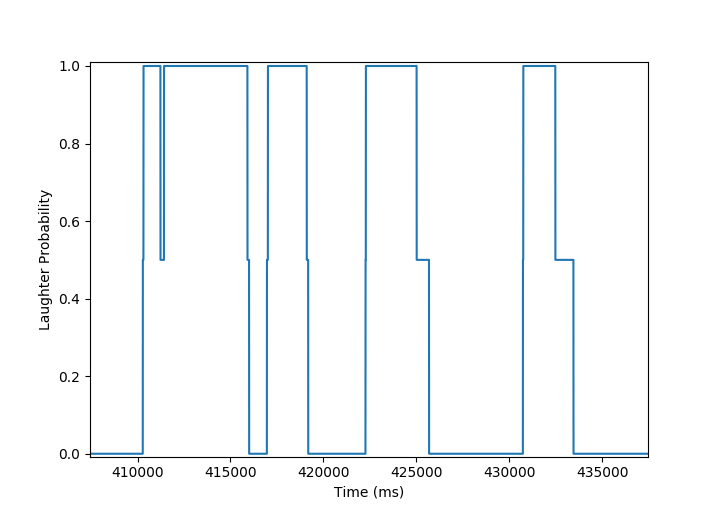
\includegraphics[scale = 0.75]{figs/differences_1.png}
	\caption{The differences in laughter classification between two different humans. Here, we see the differences in classification clearly. One classifier appears to think that laughter lasts approximately a whole second longer for the second two laughter instances, while one classifier separates the first laughter instance into two separate pieces.}
	\label{laughter_classification_differences_1}
\end{figure}
\begin{figure}[H]
	\centering
	\vspace{0.5cm}
	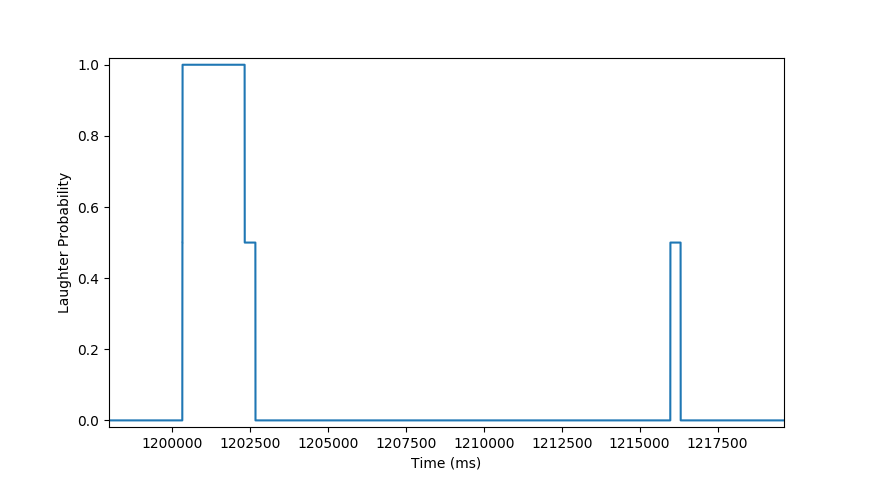
\includegraphics[scale = 0.7]{figs/differences_2.png}
	\caption{In this example, while both classifiers agree that the first laughter instance exists, only one classifier managed to find a second laughter segment.}
	\label{laughter_classification_differences_2}
\end{figure}

\noindent
The entire dataset used for training the model in this report was only classified by one person, despite the promising results and improvements enabled by multiple classifications. This was due to time constraints, and the inability to convince people to listen and classify 15 hours of speech for no apparent reward. An ideal dataset should have many classifiers, and the classification used for training could be the average of all the individual classifications. This way, a section of audio which only 50\% of people think is laughter, will only be labelled as 50\% laughter, and the sections of audio at the beginning and end of laughter segments will smoothly transition from non-laughter to laughter and back, rather than an abrupt jump.

\subsection{Preprocessing}

% Noise removal and rough volume normalisation.
% White noise removal from redacted segments.
% mfcc extraction.
	% Also talk about delta's and delta-delta's.
% The per-file normalisation of MFCC values.
% The data storage method for speed and size.
% Why did you choose MFCCs over PLPs?

There are many different transformations that the original 44kHz wave audio files must undergo before they are suitable to be used as input data for a TensorFlow model. These transformations can be separated into two parts: the preprocessing, and the TensorFlow input pipeline. Pre-processing takes place prior to any other stage, and consists of transforming the audio files into streams of features which are quickly and easily read by TensorFlow. These streams are then further transformed by TensorFlow at training-time into their final form before being used to update node weights. This latter section will be talked about in Section \ref{section:input_pipeline}. There are a few different procedures undertaken in the pre-processing stage, and this part of the pipeline is visualised in Figure \ref{preprocessing_pipeline}.

\begin{figure}[H]
	\centering
	\vspace{0.5cm}
	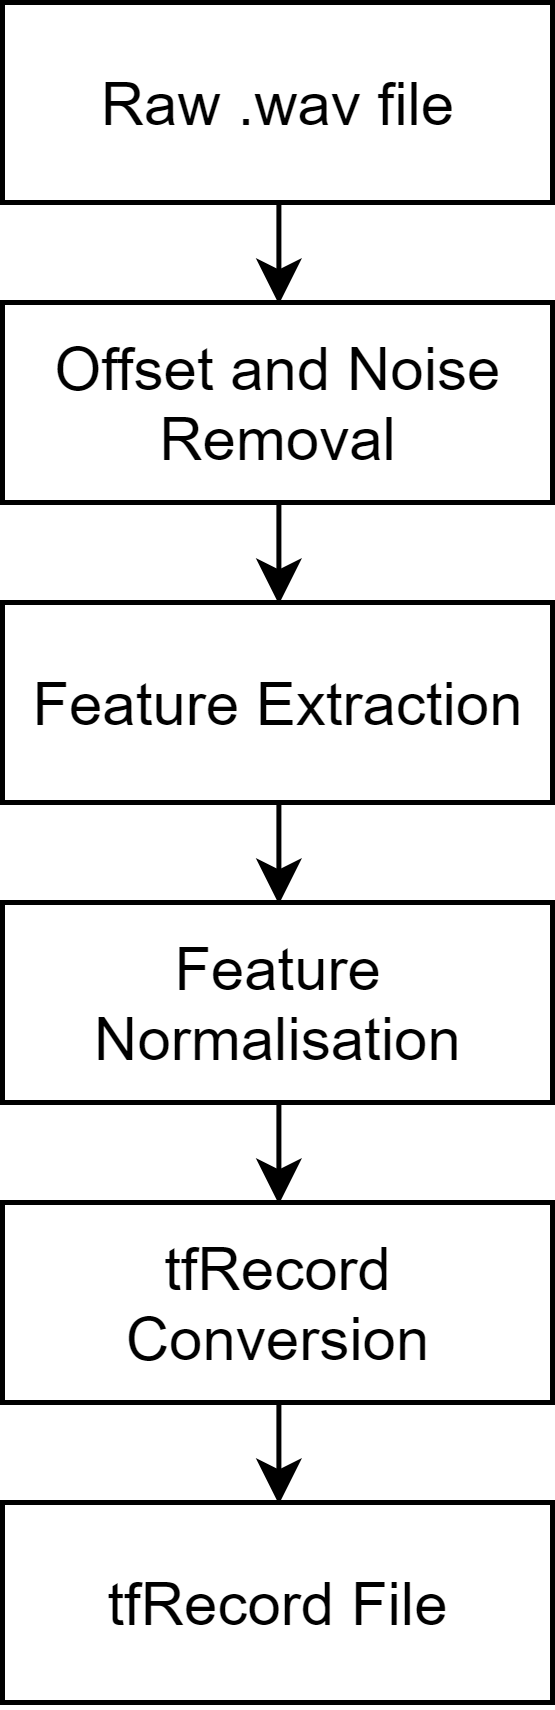
\includegraphics[scale = 0.17]{diagrams/preprocessing.png}
	\caption{The preprocessing pipeline.}
	\label{preprocessing_pipeline}
\end{figure}

\subsubsection{Volume Normalisation and Noise Removal}

Most audio files in the dataset were recorded at different times, on different recording devices, and in different locations. In machine learning, it is important to attempt to normalise all the data and to make it as similar as possible so the neural network can attempt to learn the subtle differences between what is, and isn't, laughter. This feature normalisation attempts to remove the large differences between audio files (eg, volume, pitch of speakers, noise, recording artifacts) while leaving unchanged the differences between laughter, speech, and other sounds within the audio file. Audacity was used for the first preprocessing stage, to roughly normalize the audio volume, and remove noise which persisted throughout the entire audio file.

\begin{figure}[H]
	\centering
	\vspace{0.5cm}
	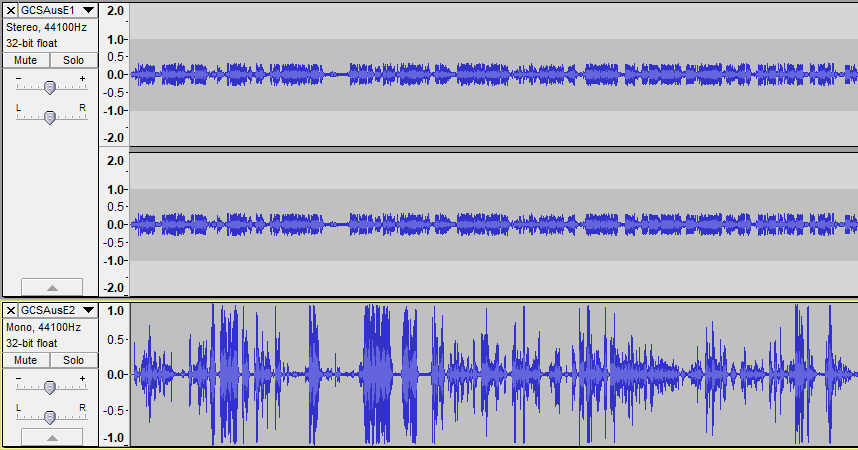
\includegraphics[scale = 0.5]{figs/origional_waveforms.png}
	\caption{The waveforms of two difference audio files before preprocessing. The top recording is in stereo, and much softer than the bottom recording. These are the differences the first stage of preprocessing attempts to remove.}
	\label{before_preprocessing}
\end{figure}

\noindent
The volume of each audio file should be roughly equal because a louder file will produce larger features. This will reduce the ability for the network to determine the actual volume of the audio in the file. The `Amplify' function in Audacity was used to boost the volume of quiet files until all audio files were roughly the same volume. This is not a precise method of normalizing the volume between different files, but the majority of this volume normalisation will be taken care of in the file-by-file feature normalization later, so it isn't important that this volume normalization is incredibly precise, only that each file sounds roughly the same.\\
\\
Next, due to the nature of this dataset, several audio files were recorded in noisy environments and had large amounts of noise distorting the audio. In this section `noise' refers to the repetitive drone of machines, electronic sinusoidal noise, and artefacts of the recording device. These types of noise are largely sinusoidal, and overlay the audio throughout the entire clip. Due to the repetitive nature of this noise, it is effectively filtered out by Audacity's `Noise Reduction' filter.\footnote{For more information on the specifics of this function, an explanation of how the algorithm works can be found here: \url{http://wiki.audacityteam.org/wiki/How_Audacity_Noise_Reduction_Works#algorithm}} This filter takes a sample of a section of the original audio file which contains only noise and no additional sounds. It takes the Fourier Transform to create a noise profile, and specifically attenuates these frequencies. This method was used to reduce the amount of noise in the original audio files, as constant sound at a certain frequency will distort to values of the features extracted from the audio.\\
\\
Lastly, the original dataset audio contained sensitive information about many locations and people who were the subject of conversation. Any names or locations have been removed from the dataset, however they have been replaced by a harsh white-noise sound. Just as other distortions will, these segments of white noise will also reduce the accuracy of the laughter detector.  Audacity was used to hand-remove as many of these segments as possible.

\newpage
\subsubsection{Feature Extraction and Normalisation}

After roughly normalizing the volume and removing noise, features need to be extracted from the audio waveform. This is a technique common to almost all speech recognition systems, and is of fundamental importance. While there are many different feature extraction methods, the features used for laughter detection were chosen to be Mel Frequency Cepstral Coefficients (MFCC's). MFCC's are essentially filter banks, measuring the intensity of audio at different frequencies. The frequency bins are scaled to imitate the ranges of audio humans hear at, and the intensity is logarithmically scaled to further imitate the perception of valume in the human ear. MFCC's were chosen because they have been used recently in a number of leading speech recognition systems.\cite{mozilladeepspeech} The number of MFCC features to generate is variable, and is generally between 12 and 26. 20 MFCC features were used in this system.\\
\\
Another feature commonly included in neural networks learning from MFCC's are their deltas and delta deltas. Training a network on MFCC's allows it to attempt to make a classification based on a snapshot of time. Deltas are the first derivative of the MFCC features, and delta deltas are the second derivative. Appending these features to the original MFCC features gives the network more information about the way the MFCC's will change in the future. Giving the network more features to train on may result in higher quality discrimination.\\
	% Additional features
	% Spanning features for non-sequential networks.
	% Clip number, feature number, labels
\\
In addition to the features listed above, the file number, sequence number, and laughter labels were appended to the list of features. The laughter labels are a one-hot encoded vector for the two different classifications: laughter, and not laughter. They are used for training in the training set, and purely for plotting against and evaluating accuracy in the test set. The sequence number refers to the nth set of features of the file. The first set of features is number 1 and is generated from the audio starting at 0.00s, and ending at 0.02 seconds. The next sequence is 2 and so on. The clip number is a unique number identifying the specific file the audio sample came from. These last two numbers, the clip and sequence number, are used in the test set when plotting the probability of the output. The clip and time in the clip when laughter occurred can be generated. This is helpful in evaluating which sounds trigger the network to recognise laughter.\\
\\
Next, each feature is normalized on a file-by-file basis. After the MFCC's for an entire file have been generated, the features are normalized accordingly by subtracting the mean of that particular feature, and then dividing by the standard deviation.
\begin{equation}
	x\prime = \frac{x - \bar{x}}{\sigma^2}
\end{equation}
Perhaps the following pseudo-code can help convey what has been done.
\begin{lstlisting}
for each 20ms frame of audio
    generate 20 MFCC's
end
save 2D value as array. Size = [number of 20ms segments, 20]

for x in 1 to 20:
    a[:,x] = (a[:,x] - mean(a[:,x])) / stddev(a[:,x])
end

// Repeat this for each file
\end{lstlisting}
This normalization further helps remove any biases, differences in volume between files, and also centres the values around zero. This is an important property of the input data for any neural network.\cite{lecun2012efficient}

\subsubsection{tfRecord Conversion}\label{section:tfRecord_conversion}

TensorFlow is used in this report to create and train the neural networks to classify laughter. TensorFlow provides a simple Python API to allow the creation of many types of neural networks with relative ease. A much more in depth discussion on TensorFlow and how it is specifically used to read data and train networks will take place in Section \ref{section:Tensorflow}, but this one important part of preprocessing occurs separate to the whole TensorFlow pipeline, and is crucial to running an efficient training pipeline.\\
\\
At this point in the pre-processing pipeline, data is saved in a two dimensional array of size: [number of frames, number of features]. A primitive method of saving this array for use by TensorFlow would be to use a comma separated variable file (CSV). This saves all numbers and variables as UTF16 variables. This is human-readable and neat, but very computationally inefficient. To read any single set of features from the table, the entire line must be parsed by a CSV reader, stacked into a Tensor, and parsed to the next stage of the input pipeline. This is orders of magnitude slower than reading a binary file, and if more complex reading is needed, column by column for example, CSV files become even more inefficient. Google recognised this when creating TensorFlow and created a custom binary data type called tfRecords which can be used for data storage.\\
\\
TfRecords have the ability to store many different data types in the same file as a sequence of binary strings. It is similar to HDF5 (Hierarchical Data Format) which is designed to store and organise large amounts of data efficiently, but with a few extra features built in. TfRecords contain sets of key-value `features' where the key, (a string) maps to binary data which can be many different data types. Reading this data is fast, and the hierarchical format leads itself to being organised into Tensors quickly and efficiently.\\
\\
Consequently, the final stage of the preprocessing pipeline is to convert every audio file's set of features into a tfRecord file for fast accessing by TensorFlow. Adding this step increased the training speed of the network by an order of magnitude and simultaneously reduced the file size by $\sim$20\%.

\subsection{Initial Analysis}

Before taking the large laughter database straight to TensorFlow, it is useful to attempt to visualise differences in our features before trying anything more complex. For example, if we can show that laughter is easily separable just by observing feature values, why bother going to all the trouble using neural networks if this problem can be solved another way. In reality, it is expected that there will be no simple way to discriminate between laughter and non-laughter, because if there way, problems like speech detection would have been solved a long time ago. It is still useful however, as it will give a `feel' for the data, which may help when building a more complex network.\\
\\
Simply looking at the audio waveform for examples of audio and laughter is a good place to start.

\begin{figure}[H]
	\centering
	\vspace{0.5cm}
	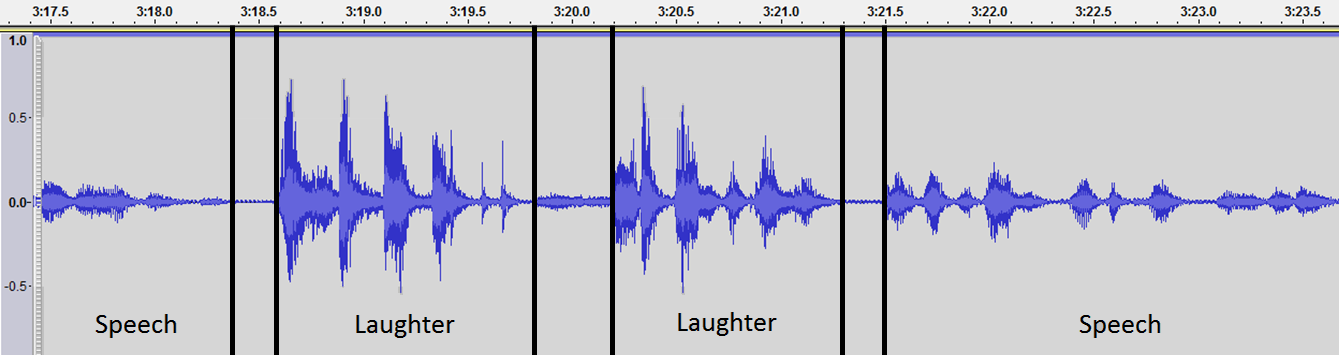
\includegraphics[scale = 0.4]{figs/time-series2.png}
	\caption{The time series waveform of an audio sample containing both laughter and speech.}
	\label{time-series2}
\end{figure}

\begin{figure}[H]
	\centering
	\vspace{0.5cm}
	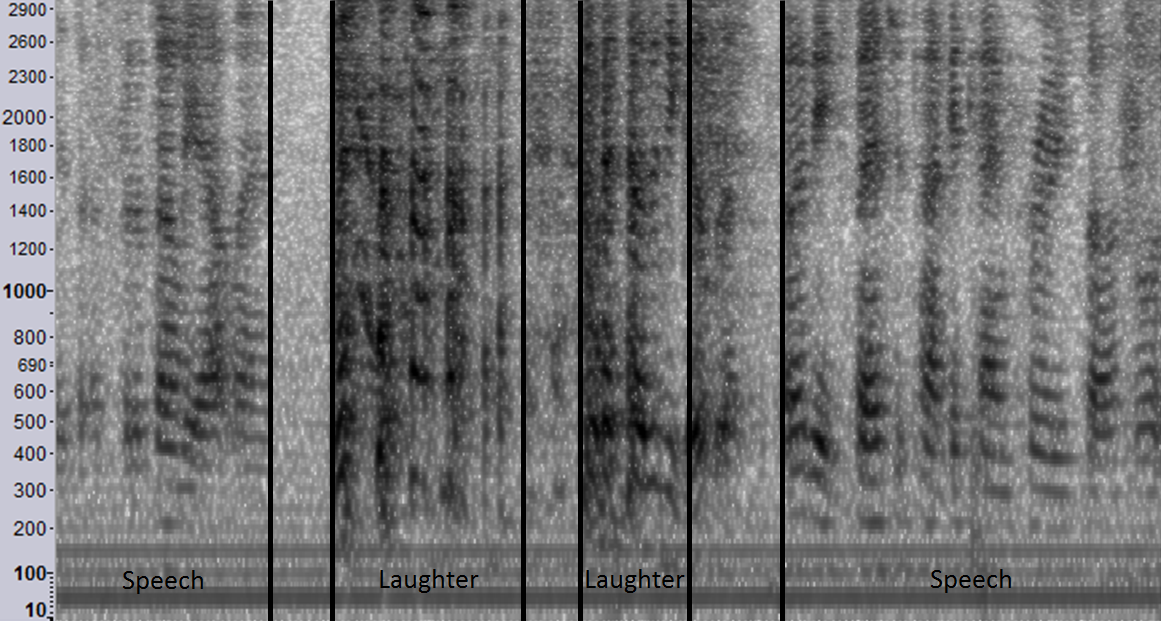
\includegraphics[scale = 0.462]{figs/spectrum2.png}
	\caption{A spectrogram visualisation of the same waveform shown in Figure \ref{time-series2}.}
	\label{spectrum2}
\end{figure}

\noindent
The waveforms shown in Figure \ref{time-series2} and Figure \ref{spectrum2} both show the waveforms of laughter and speech in different ways. There are differences between them visually in both representations, but there are no defining features of either one. In the time series waveform, the laughter appears to be louder than surrounding speech, and in the spectrogram visualisation, the finer harmonic details in speech appear to be lost, or at least much more complicated in laughter. Either way, this audio sample is interesting and shows some differences, however the dramatic differences in laughter can actually sound like make this a significantly harder problem. Laughter is not always louder than speech however, so creating a system that purely recognises volume would miss-classify loud speech and soft laughter.\\
\\
These waveforms convey some different features, however the neural network trained on this dataset isn't trained on the full waveform data used to generate these pictures, but on the normalised MFCC features previously generated. In order to visualize these MFCCs, lets plot that same section of audio again, but this time look at the normalised MFCC features.

\begin{figure}[H]
	\centering
	\vspace{0.5cm}
	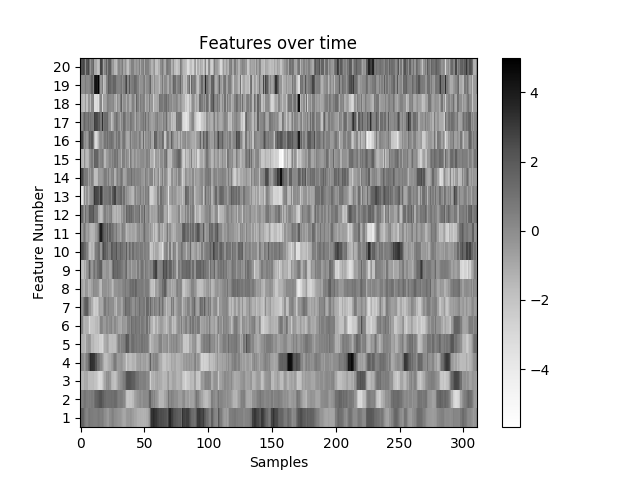
\includegraphics[scale = 0.8]{figs/features_visualisation_grey.png}
	\caption{The same 6 seconds of audio as Figure \ref{time-series2}, and Figure \ref{spectrum2}, but in MFCC feature form.}
	\label{mfcc-visualisation}
\end{figure}

\noindent
This plot shows that the normalized MFCC values from this small audio clip differ greatly from the spectrogram in Figure \ref{spectrum2}. The general magnitude of the audio can be seen in the first MFCC feature, showing two darker sections. All other features tend not to change hugely over the audio clip. From this plot, it is definitely not possible to easily tell the difference between laughter and non-laughter.\\
\\

% This is performing PCA and t-SNE on the origional data and features.
\noindent
Another method of visualising the features from the audio is to use the t-SNE algorithm to see if there is any relation between laughter segments \cite{maaten2008visualizing}. The t-student Stochastic Neighbour Embedding (t-SNE) algorithm is a dimensionality reduction technique used in machine learning to help visualise multi-dimensional data.\footnote{The creator of the t-SNE algorithm, Laurens van der Maaten, has published code to implement the t-SNE algorithm in several different languages on his website: \url{https://lvdmaaten.github.io/tsne/}. His code was used to generate these t-SNE plots.} t-SNE works by attempting to preserve distances between points in a higher dimensional space, and the lower dimensional space. It does this by plotting all points randomly on a two dimensional plane, and moving them according to forces placed on them by neighbouring points. These forces are proportional to the distance between points in their higher dimensional representation. Using t-SNE the reduce the 28x28 pixel features of the MNIST handwritten digit dataset to two dimensions, separates the different digits almost perfectly. If there are any similar features between audio files, or between different sounds, it is expected that they cluster together.

\begin{figure}[H]
	\centering
	\vspace{0.5cm}
	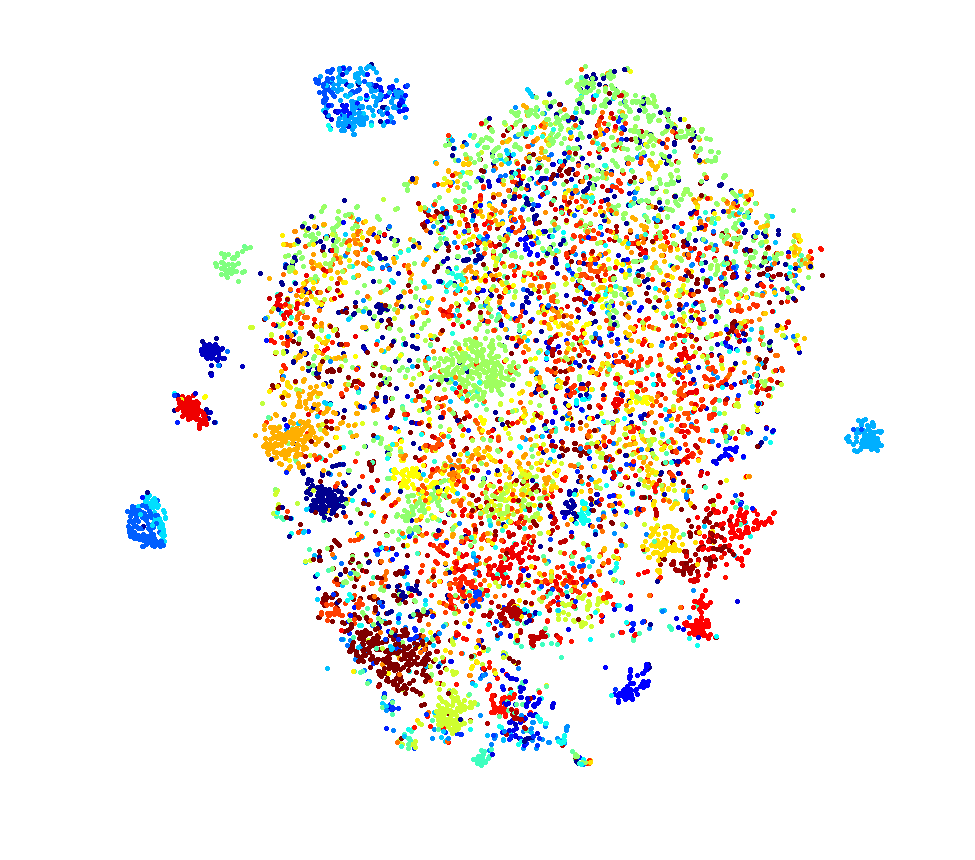
\includegraphics[scale = 0.65]{figs/tsne2.png}
	\caption{t-SNE plot of a randomly selected set of frames of features from un-normalized MFCC's. Frames are coloured according to the file they belong to. Several clusters containing points from the same audio file can be seen.}
	\label{tsne_unnorm}
\end{figure}

\begin{figure}[H]
	\centering
	\vspace{0.5cm}
	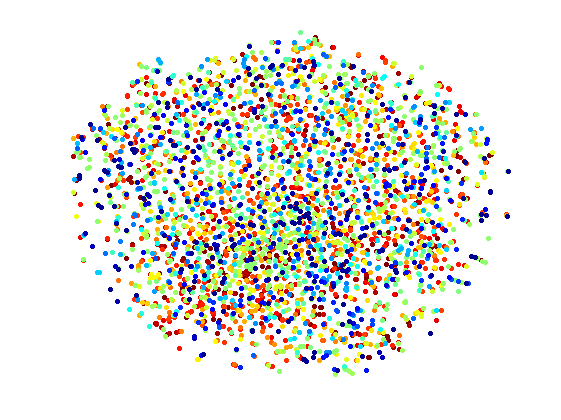
\includegraphics[scale = 0.75]{figs/tsne_normalised.png}
	\caption{t-SNE plot of a randomly selected set of frames of features from normalized MFCC's. The clustering of points mostly disappears when normalising all the features.}
	\label{tsne_norm}
\end{figure}

\begin{figure}[H]
	\centering
	\vspace{0.5cm}
	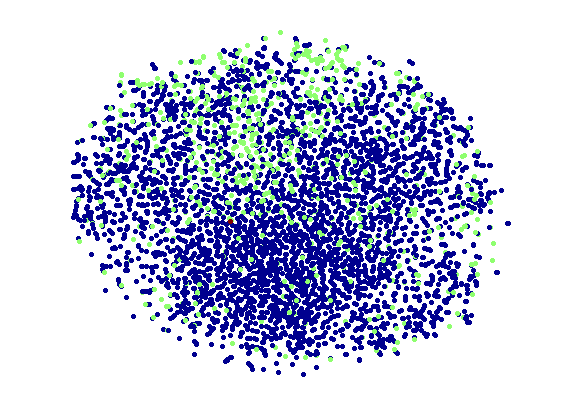
\includegraphics[scale = 0.75]{figs/tsne_normalised_with_laughter.png}
	\caption{This figure shows the exact same plot as Figure \ref{tsne_norm}, but the points are coloured according to whether they are laughter or not, not according to their original file. Blue points represent frames of non-laughter, and light green represents laughter.}
	\label{tsne_norm_laughter}
\end{figure}
\clearpage

% Show that the data doesn't really appear to be especially seperable.
\noindent
In Figure \ref{tsne_unnorm}, large clumps of similar coloured points form together. These points are all random points from the same file. The obvious outliers around the outside of the largest cluster all come from files with large amount of background noise. This background noise that features throughout the file are present in all frames of the file, and give them very different features compared to audio from other files. This is not a good thing for creating a neural network, because all audio files should be roughly `the same' in that they contain human speech at roughly the same volume. Some parts of the audio files will be louder than others, but on average, the files should be roughly the same volume, contain the same features, and be roughly similar. In order to get rid of this, and attempt to normalise all the files, the features from each file were normalised. Plotting this gives Figure \ref{tsne_norm}, where it can be seen that there are no more outlying clusters, and all points seems to be roughly evenly distributed in a single cluster. This shows that the normalisation of the files has worked, in that now each file is no longer easily identifiable by these unique noise features. Figure \ref{tsne_norm_laughter} shows this same plot again, with the laughter coloured green, and the non-laughter blue. There are no obvious clusters, but it can be seen that the laughter segments do seem to mainly lie at the top of the cluster. From this, it would appear that laughter should be slightly separable from non-laughter, and a classifier with above random accuracy should be able to be created.

% Matlab Neural networks.
\subsection{Matlab}\label{section:Matlab}
After creating features from the audio in Matlab, the Matlab Neural Network Toolbox could be used to quickly create a network and train it on audio to attempt to detect laughter. Creating a neural network with a variable amount of layers, and quickly training it is especially easy with this toolbox. Some parameters are able to be changed easily, such as the dimensionality of the data, the number of layers and activation functions, and the type of regression. However, Matlab's toolbox has been created to enable a programmer to quickly create a model, not to give absolute control over the architecture of the network. On top of this, Matlab's neural network toolbox has no support for datasets larger than the allowed memory of the computer, and attempting to train a network on more than 10\% of the total audio data causes errors.\\
\\
In saying this, for only training on a couple files, the networks Matlab created were pretty good, and could detect laughter at an above-random rate. It was impossible to test the full accuracy of a model, as Matlab could not load the full dataset at once, but it could visibly classify laughter.

\begin{figure}[H]
	\centering
	\vspace{0.5cm}
	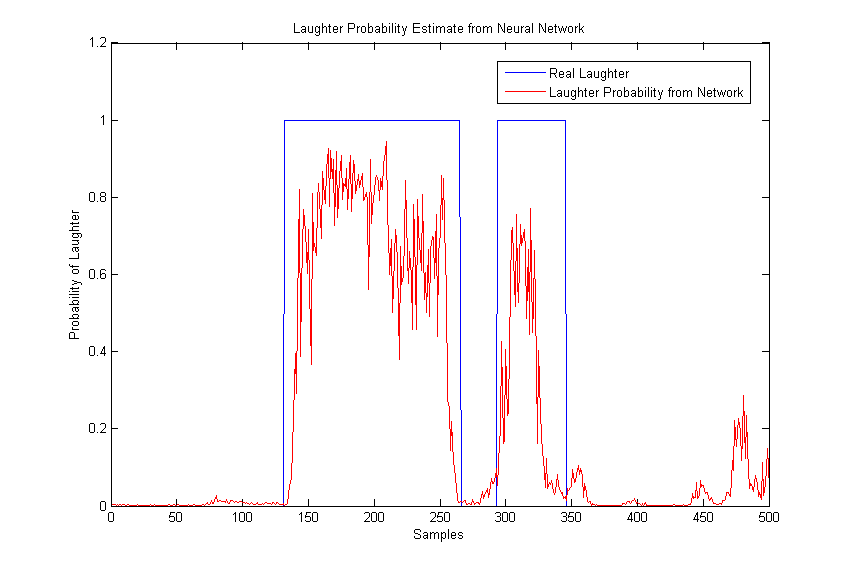
\includegraphics[scale = 0.6]{figs/prob_of_laughter.png}
	\caption{A graph of the probability of a section of audio being laughter, as created by the Matlab Neural Network Toolbox. It is plotted with the truth values, to show which areas are laughter, and which are not. This is an example of the network performing well.}
	\label{matlab_nn_probability}
\end{figure}

\noindent
In short, Matlab's network is fantastic for what it was created for, to quickly create neural networks, but it does not allow the same level of control over the system as TensorFlow does. Due to Matlab's inability to train on more than a couple audio files at once, and the need for more network customisation options, TensorFlow was used to create a much more detailed network for laughter classification.

\subsection{TensorFlow}\label{section:Tensorflow}

% What tensorflow is, and why I chose to use it over something like MATLAB.

TensorFlow is an open source software library which allows programmers to implement complex machine learning algorithms with relative ease. TensorFlow contains functions to perform efficient n-dimensional matrix (tensor) manipulating and calculation, by building a graph of mathematical functions which the tensors `flow' between. By generalizing these operations to nodes of a graph, general gradient calculation for back propagation through neural networks can be done with a single function, allowing any confident programmer to fiddle with these networks and use them to train intelligent systems on almost anything. It also supports many other complex features such as: deployment on mobile devices, GPU acceleration, and scalable distributed training and testing across multi CPU/GPU systems. Since it is open source, it also features complex and state of the art systems contributed by leading researchers in their fields \cite{tensorflow2015-whitepaper}.\\
\\
TensorFlow was chosen as the program to be used in this project, over other competing programs such as MATLAB's neural network toolbox, scikit-learn, Caffe, and many others, because of its lower level implementation and the finer control it provides. In addition to this, it is open source, has copious documentation, and will allow the quick and effortless prototyping of many different types of neural networks with different parameters. TensorFlow is also packaged with TensorBoard, a network visualisation tool, allowing the network architect to visualise the network's node weights, accuracy, cost, and any other feature instantly and effortlessly. Initially MATLAB's neural network toolbox was trialled, however it lacked the basic functionality to support datasets larger than the total amount of memory available to the system. This would have made training the laughter detector impossible, so the switch was made to TensorFlow immediately.

\subsubsection{Input Pipeline}\label{section:input_pipeline}

% Talk about the many different input pipelines I've tried but mainly:
	% The frame by frame batches
	% The sequences of frames batches.
	% Remember to insert pictures of the networks from tensorboard.
The input pipeline for the TensorFlow model was the most reworked and optimised section of code in this entire project. The input pipeline contains all code for processing input data from storage on disk, into memory, and finally through the network. If not done efficiently, and input data is supplied slower than it can be processed by the network, the input pipeline can be a bottleneck for the entire program. On top of this, TensorFlow is mid-way through rolling out a new (more efficient) API for input pipelines, which contains limited documentation, making this part of the program quite difficult.\\
\\
The goal of an input pipeline is to:
\begin{itemize}
\item Transform input data into tensors for training
\item Generate input batch-by-batch, not loading the whole dataset into memory at once
\end{itemize}
This second point allows TensorFlow to surpass Matlab's toolbox by allowing us to train a network on the entire dataset.\\
\\
Another purpose of the input pipeline is to create batches. Batches are collections of a number inputs, for which gradients are calculated. These gradients are then averaged and applied to the weights of the network in a single update step. Batching presents a large improvement in speed by allowing the gradients for several hundred inputs be calculated in parallel, and applied at once. The downside to batching is that gradient updates will capture the general features of the data, but the error from any one-off frames will be averaged with many others and not effect the node weights as strongly as it may have if it was calculated separately. For this reason, it is generally recommended that the smallest possible batch size is used, to allow the system to train in a reasonable amount of time. A batch size of around 500 sequences was used in final models as it gave a balance between speed and accuracy.\\
\\
The initial versions of the input pipeline read data from a Comma Separated Variable (CSV) file, and read lines into tensors, batched, and shuffled the data, and fed it into a model classifying individual frames as laughter or not. It did so using TensorFlow's old input pipeline model, which is a series of queues, and threads which dequeue data from one queue, perform an operation, and enqueue it into the next queue. This creates a pipeline of queues which data flows though. It also allowed the length of the queues to be monitored in real time, so bottlenecks could be found. The major bottleneck with this approach was the use of CSV files. Once the CSV files were replaced with TfRecord datasets, the whole process ran much faster for reasons explained in Section \ref{section:tfRecord_conversion}.\\
\\
The most recent and successful laughter detection methods used a `context window' of frames entered into the network to detect laughter. A `context window' here is just a series of frames in sequence which enter the network simultaneously. After all, a human most likely can not detect laughter in an audio clip 20ms long, but rather needs a sequence of frames to make a decision on. Creating a dataset of these sequences could be done in a number of ways:
\begin{itemize}
\item Create a script to transform the dataset into a number of sequences, and store on disk
\item Dynamically form sequences from original data
\end{itemize}
For neural networks, the training data is very important. For this reason, when creating the sequences, we don't want to throw away any data. For example, lets imagine an audio file containing 1000 20ms long frames. If we wish to create a number of sequences from this audio, each with 50 frames (so that each sequence is 1 second long), then we can either separate the 1000 frames into 20 sequences of 50, where each sequence is 100\% unique, or we can slide the window over by a single frame for each sequence, creating 951 different sequences. The second option retains the most information from the original sequences, and is also used by other laughter detection papers, so this is the method which was used. If a script was used to create a dataset using this method, it would bloat the size of the dataset stored on disk to almost 50 times as large, and reading hundreds of gigabytes of data is not ideal. TensorFlow's old input pipeline method didn't allow easily mapping tensors from one shape to another, but their new Dataset API allows creating mapping functions, so the pipeline was modified to use this API. The process of creating these batches of sequences of frames is illustrated in Figure \ref{sequence_generation_mapping}, and the TensorFlow graph of this input pipeline is shown in Figure \ref{input_pipeline_graph}.

\begin{figure}[H]
	\centering
	\vspace{0.5cm}
	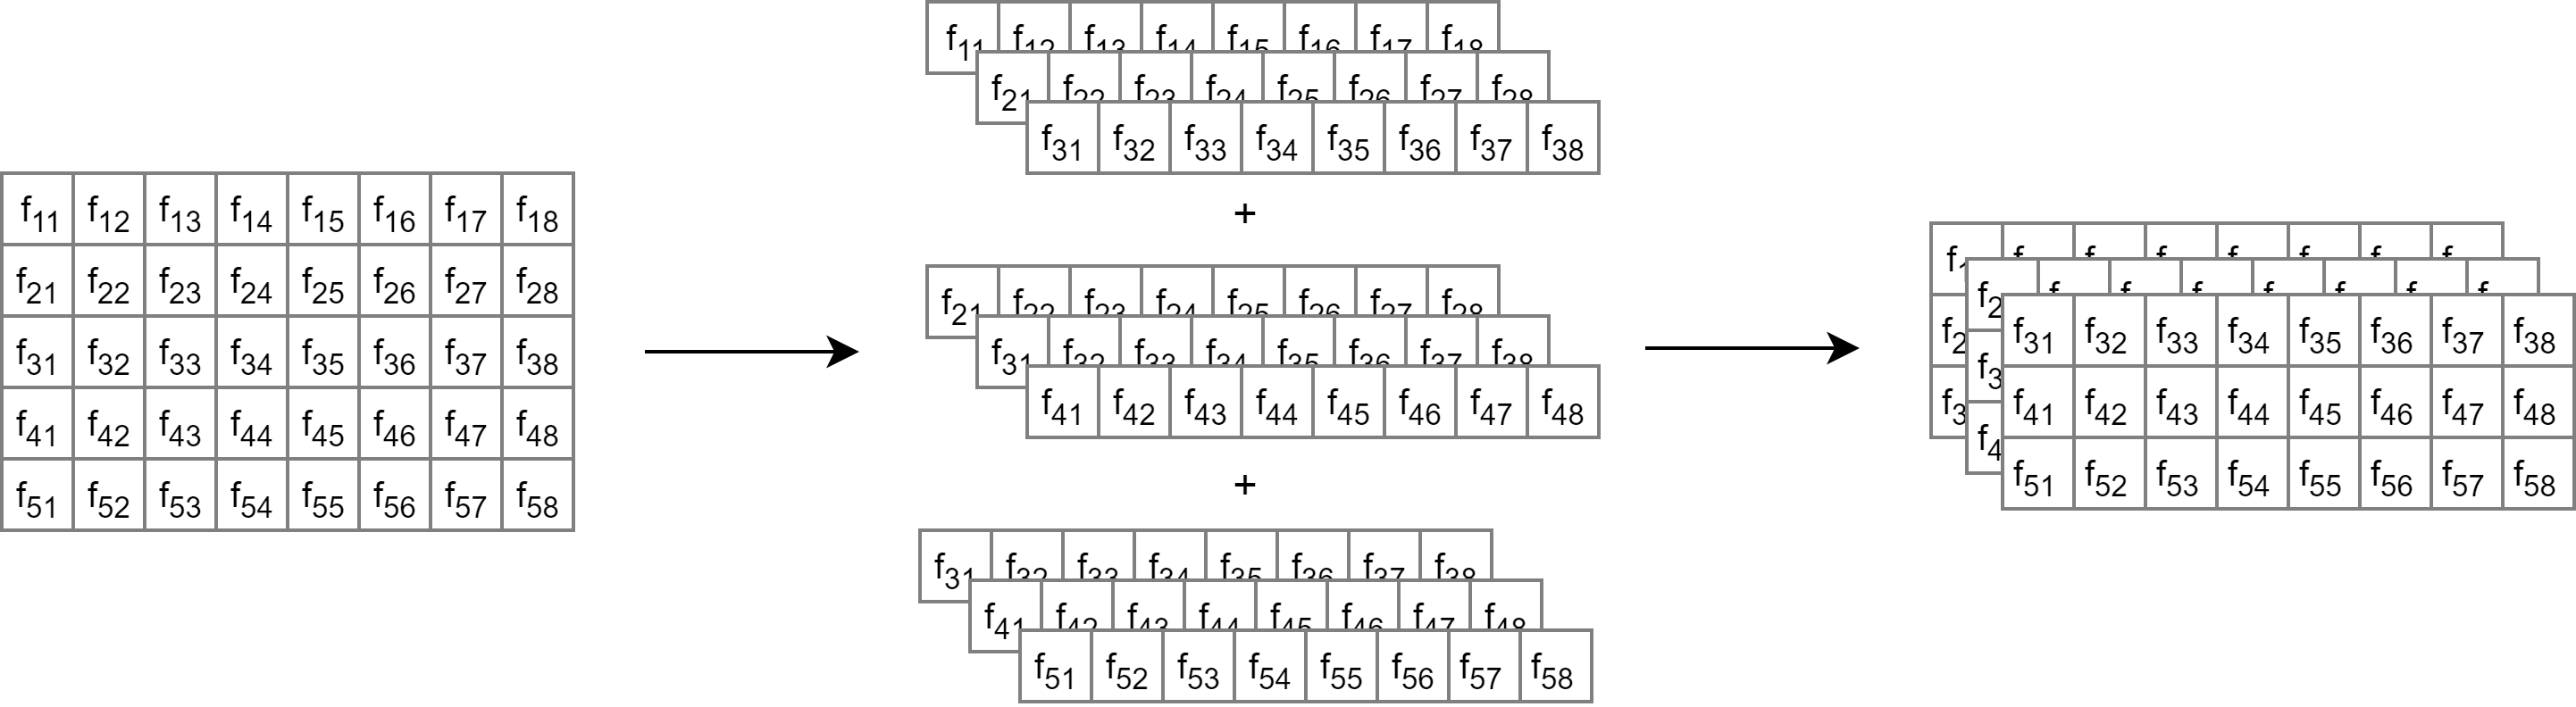
\includegraphics[scale = 0.15]{diagrams/sequence_generation.png}
	\caption{A diagram showing a visual representation of the mapping used to generate sequences for a neural network expecting sequences. The original format on the left is two dimensional, with the different features along the x axis, and the different frames along the Y. This is transformed into the three dimensional tensor on the right, with features on the X axis, different sequences on the Y axis, and the frames which make the sequences on the Z axis.}
	\label{sequence_generation_mapping}
\end{figure}

\begin{figure}[H]
	\centering
	\vspace{0.5cm}
	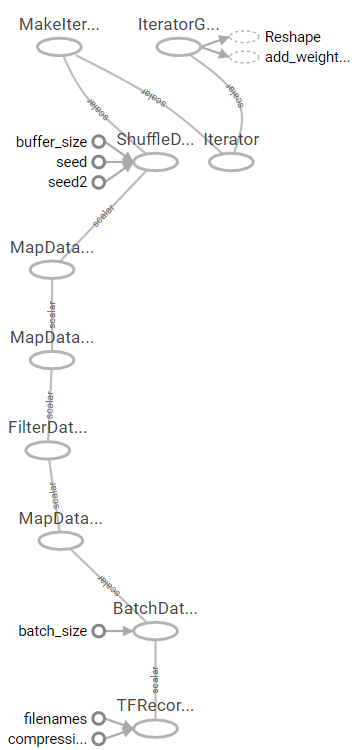
\includegraphics[scale = 0.75]{figs/input_pipeline_graph.png}
	\caption{The input pipeline graph created in TensorFlow. It reads from the bottom to the top. The bottom node reads TFRecords, followed by a series of nodes, batching, mapping, filtering, and shuffling the data many times before creating an iterable tensor variable the network can pull data from.}
	\label{input_pipeline_graph}
\end{figure}

\noindent
Now that sequences have been generated, another important question to ask is: ``If we have a sequence which is half speech, and half laughter, what is it labelled as?'' This problem has been solved in this study by assignment the label of the centre frame of the sequence to the sequence in question. In short, if the frame of audio in the centre of the sequence is laughter, then the entire sequence is classified as laughter. This was experimented with, and it was found that if the first or last frame was considered the truth label of the sequence, the model with predict laughter either too late, or two early respectively.

\subsubsection{Models}

% Talk about all the various TensorFlow models I attempted to use.
	% mlp
	% sequence mlp
	% ltsm
% Talk about additional features of the networks
	% Dropout
	% Batch normalisation
	% Shuffling
	% Activiation Function
		% Relu clipping

After creating an input pipeline to perfectly pass tensors from disk into a network, it is time to create the network. The first created networks were simple multi-layer perceptrons (MLPs) which imitated the networks from the Matlab toolbox. This type of network is illustrated in Figure \ref{mlp_example}.

\begin{figure}[H]
	\centering
	\vspace{0.5cm}
	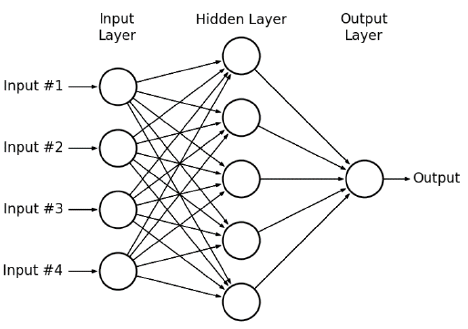
\includegraphics[scale = 0.75]{figs/mlp.png}
	\caption{A diagram of a simple MLP. Much like our system, it contains a single hidden layer however our system has two output nodes, 20 input nodes, and 400 nodes in the hidden layer.}
	\label{mlp_example}
\end{figure}

\noindent
Helper functions were created to abstract the process of creating the graph representing the neural network, allowing the quick creation and testing of networks with different numbers of layers, numbers of nodes, activations functions, and other features. This let hundreds of different networks be tested to determine which has the highest accuracy of laughter classification.\\
\\
Two main networks were tested in this report, the MLP which classified single frames, and the larger MLP which classified a whole context window of input features. The accuracy of both of these will be mentioned in the results section of this report. A third network utilising long-short term memory units was attempted using TensorFlow, however after training numerous models with it no reasonable results were obtained. Not enough is known about LSTMs to know whether this was due to an incorrect training method, incorrect system, or other issues. Either way, the results obtained from LSTM models will not be discussed further.

\begin{figure}[H]
	\centering
	\vspace{0.5cm}
	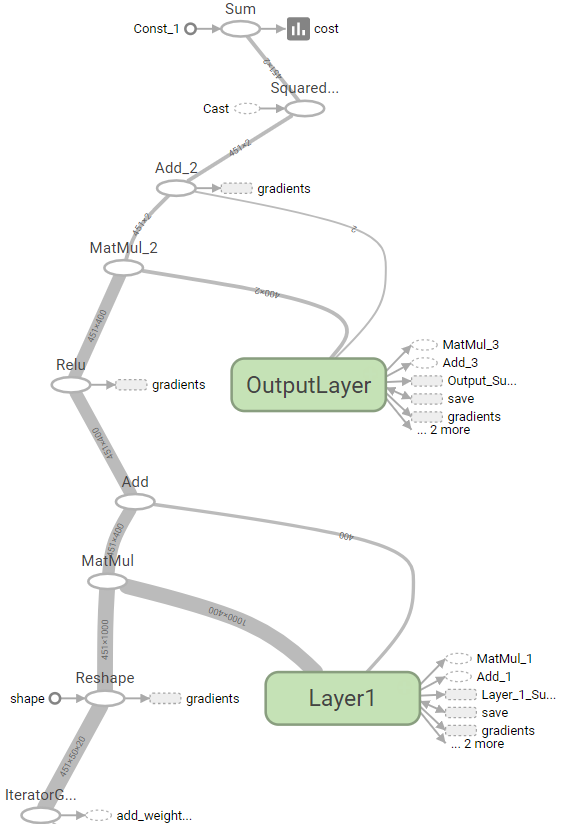
\includegraphics[scale = 0.70]{figs/network_diagram.png}
	\caption{The TensorBoard graph showing the flow of tensors from the end of the input pipeline through a series of additions and multiplications by the weights stored in the layers of the neural network to the cost function at the outputs.}
	\label{network_diagram1}
\end{figure}

\begin{figure}[H]
	\centering
	\vspace{0.5cm}
	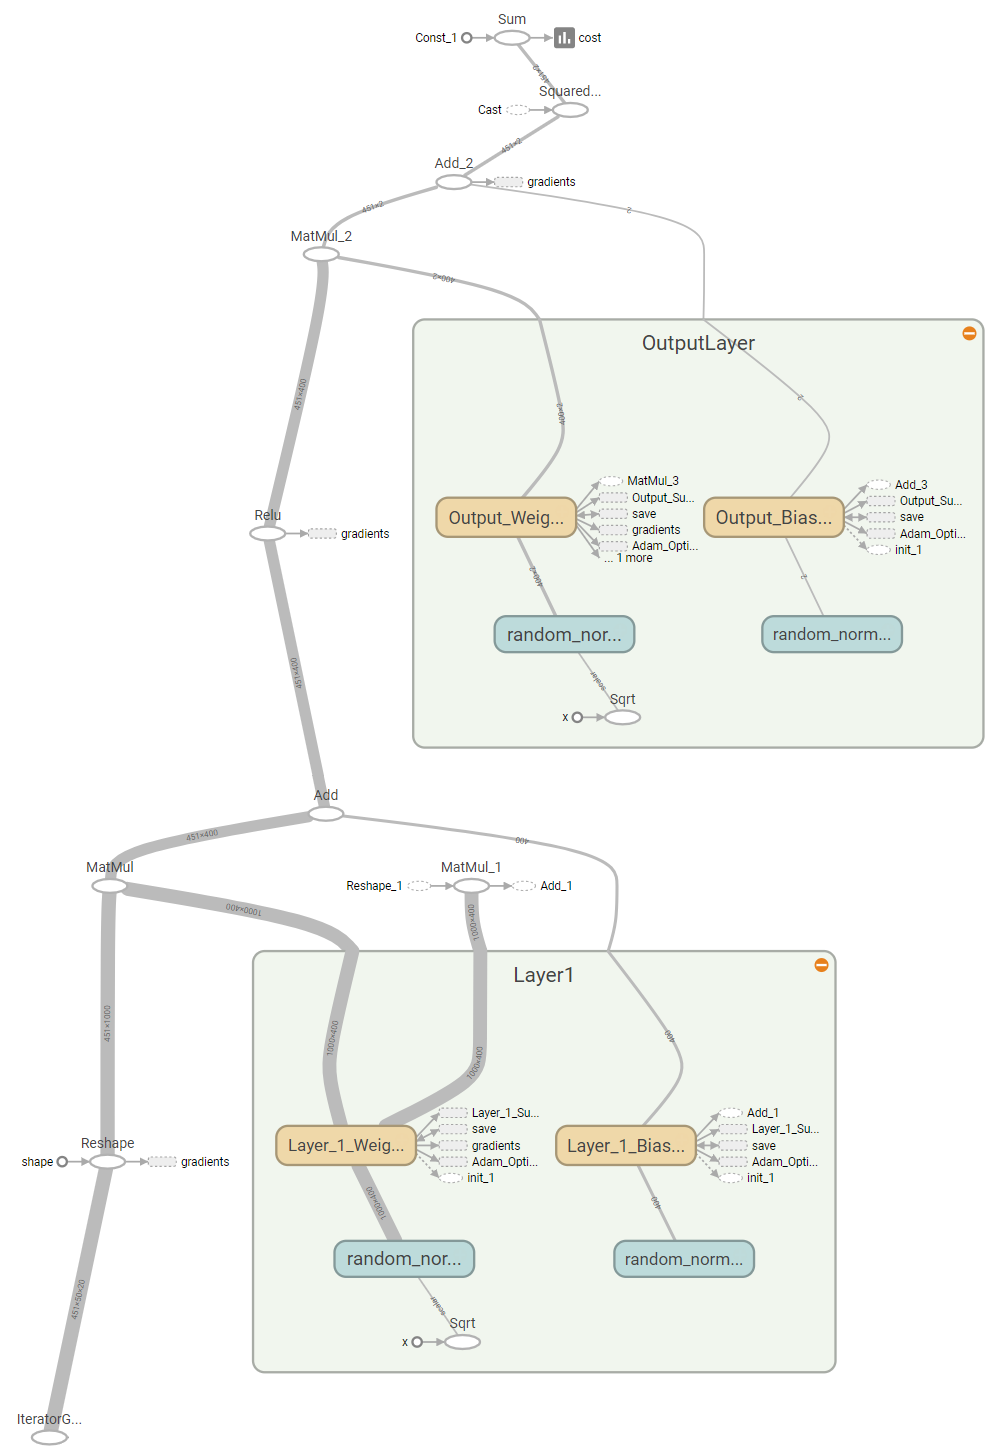
\includegraphics[scale = 0.5]{figs/network_diagram3.png}
	\caption{A diagram similar to Figure \ref{network_diagram1} with expanded layers, showing the variable initialisation and connections between variables and their calculated gradients.}
	\label{network_diagram2}
\end{figure}

\newpage
\subsubsection{Initialization}

% Talk about initialization of the network.
	% Xavier Initialisation
Another important part of network creation is the initialisation of node weights. If all node weights were initialised as 0, all nodes would change according to the same gradient, and the network would perform equivalent to having a single node. To break this symmetry, all nodes weights are initialised according to a random variable. The distribution of this random variable effects the results of the network greatly.\\
\\
Initially, the easiest way to initialise the weights was to select them from a normal distribution. This is a Gaussian distribution centred around zero, with a standard deviation of 1. The laughter probability results from such a network were either 100\% or 0\% as shown below in Figure \ref{bad_initialisation1}, and did not display nice transitions between them as seen in Figure \ref{matlab_nn_probability}.

\begin{figure}[H]
	\centering
	\vspace{0.5cm}
	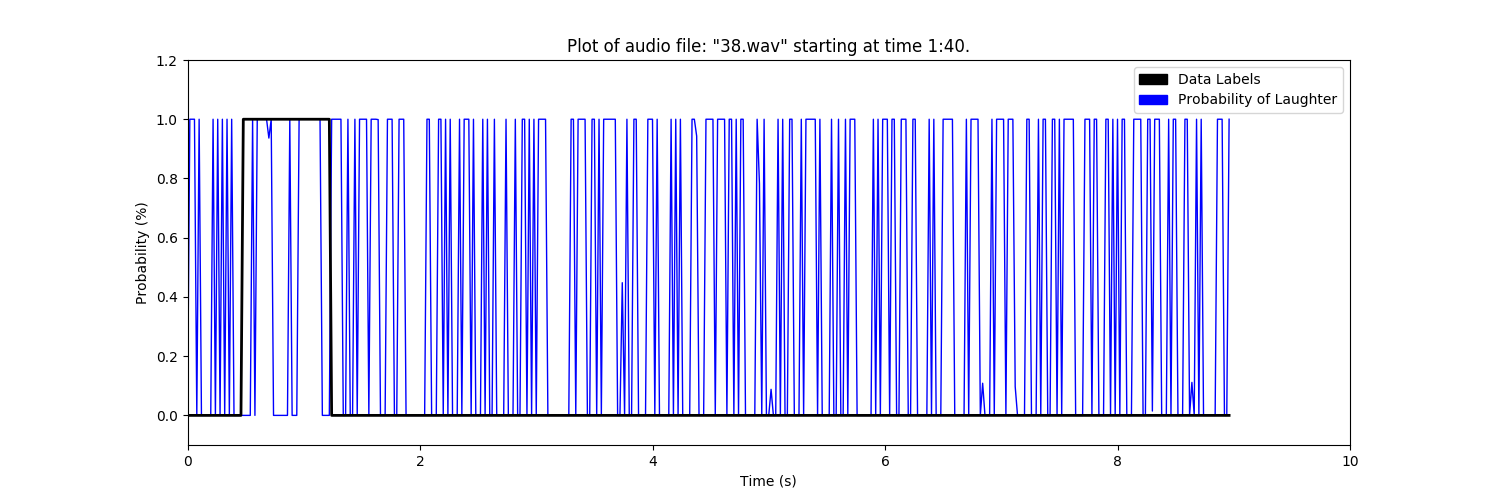
\includegraphics[scale = 0.4]{figs/bad_initialisation1.png}
	\caption{The probability of each sequence being laughter when the nodes are initialised to large values. While the network does appear to be learning, and the accuracy is better than random, not having values between 0\% and 100\% stops us from being able to change the threshold for laughter to change the number of false positives and false negatives.}
	\label{bad_initialisation1}
\end{figure}

\noindent
Through researching this problem, a solution is using Xavier initialisation to initialise nodes. This method was first published in 2010 by Xavier Glorot, and Yoshua Bengio \cite{glorot2010understanding}. They discovered that if you look at the output of a linear neuron, you can write it's output like so:
\begin{equation}
Y = W_{1}X_{1} + W_{2}X_{2} + \ldots + W_{n}X_{n}
\end{equation}
Now, if you assume that both $X$ and $W$ are distributed about 0\footnote{This is another reason why it is important to normalize input data about 0.}, then the variance of the output for an initial uniform distribution of node weights is:
\begin{equation}
Var(Y) = Var(W_{1}X_{1} + \ldots + W_{n}X_{n}) = n\times Var(W)Var(X)
\end{equation}
So the variance in the output is proportional to the variance of the input and initial weights, and the number of nodes in the layer. Since our system used large numbers of nodes in the hidden layer, in order to maintain a constant variance, the standard deviation of the initial node weights in the hidden layer need to be reduced. For Gaussian distributions, and different activations functions, these calculations are slightly different. Dividing the standard deviation by some proportion of the number of nodes in the hidden layer fixes the problem, and gives outputs as shown in Figure .

\begin{figure}[H]
	\centering
	\vspace{0.5cm}
	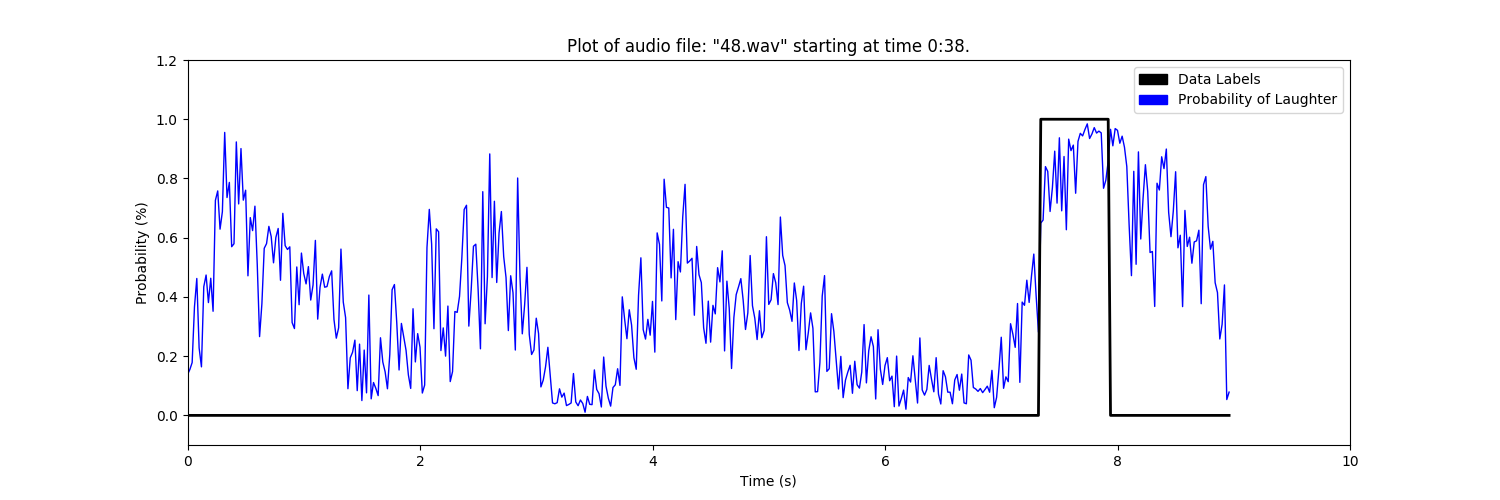
\includegraphics[scale = 0.4]{figs/good_initialisation1.png}
	\caption{The probability of each sequence being laughter when nodes are initialized according to a Gaussian distribution with variance specified by Xavier initialisation.}
	\label{good_initialisation1}
\end{figure}

\subsubsection{Cost Function}

% Talk about the cost function I used. Maybe put this in the previous section or something.
% Specifically how adding the extra cost to the laughter segments changes the ratio at which they are classified.
The gradients which define the weight updates of the neural network are calculated in order to minimise the cost function. TensorFlow makes the computation of these gradients incredibly easy, as you can compare the computed values to the actual values, generate some number for the error between these values, and tell TensorFlow to generate gradients to minimise this number. Due to the graph-like nature of TensorFlow computation, the derivatives at each node can be calculated, combined with the chain rule, and the ideal gradient for the weight update can be found.\\
\\
To calculate the cost function for this dataset, two different methods were used:
\begin{itemize}
\item Mean Squared Error
\item Softmax Cross Entropy
\end{itemize}
% Paragraph on mean squared error
The mean squared error is a more standard error calculation method, where you square the difference between the prediction and the actual value, and find the average for this calculation for each sequence in a batch. This cost function attempts to force the outputs of the network towards the correct values, and squaring the error `punishes' the network much more for larger errors.\\
\\
% Paragraph on softmax cross entropy
The softmax cross entropy cost function was also tested yielding different, but not necessarily better, results. This cost function calculates the cross entropy between the labels, and the predictions, and in certain circumstances performs better than the mean squared error \cite{dunne1997pairing}. Rather than simply squaring the difference, this function looks like this:
\begin{equation}
C = -\frac{1}{n}\sum_{x}(y\ln a+(1-y)\ln(1-a))
\end{equation}
Here, $C$ is the cost, $a$ is the predicted output, $y$ is the actual label, and $x$ is the number of features in the batch. This function solves learning slowdown when using sigmoidal activation functions, and results in very different node weights compared to the mean squared error cost function.\\
\\
% Paragraph on the hacky way I fixed the missmatch between the number of laughter and non-laughter sequences.
Another large problem of this system, is the mismatch in sizes of data from each class. In over 15 hours of audio, if all the laughter segments were cut out and joined together, they would last just over 20 minutes. This is a data size discrepancy of approximately 40 times. If this dataset is simply ran through the network, there will be 40 times more batches which tell the network that the correct answer is `non-laughter', and all nodes will be trained that if they answer `non-laughter', they will be correct most of the time which minimises the cost function. This makes sense, because 97\% accuracy can be achieved with this dataset if the network simply answered `non-laughter' to every piece of input data. This is obviously not the purpose of this study however, as the network should be learning the laughter. There are two ways commonly used to fix this dataset size mismatch problem:
\begin{itemize}
\item Make the amount of data for each classification option equal
\item Modify the cost function to favour a certain classification
\end{itemize}
The first option here involves either throwing away a large amount of non-laughter audio, or more commonly, duplicating laughter segments. This can be done either in dataset creation, or in the input pipeline in TensorFlow. However, this would be tricky and there are no inbuilt functions for duplicating data specific numbers of times in the input pipeline of TensorFlow and would need to be created by hand. The other option here is much easier, modify the cost function to more heavily penalize the misclassification of laughter sequences. In the cost function, if a multiplier is added to the cost of all the laughter segments, it forces the network to classify laughter and non-laughter segments more equally.\\
\\
Using this method of dataset size normalizing has it's problems too. Since laughter segments come in series, often batches will either contain no laughter sequences, or many laughter sequences. This causes the batches to either have a very low cost, or a very high cost. This then creates either very small or large gradients, which result in very small or large node weight changes. Ideally, the nodes are changed a very small amount every update, and the size of these weight updates can be controlled with the learning rate constant. This is set small enough to stop training instability. However, if some updates are large, and others are small, then to ensure the system's weights are not being constantly thrown around by large weight updates, the learning rate must be set very low, and this causes training to take a long time.

\newpage
\subsubsection{Training}

% Talk about my training methods and how I split data and train on it.
	% Not so much because it's interesting or unique, but to show I did it correctly.
% Talk about not using a validation set, and the effects of that. Also, what I did to try to mitigate the effects of this.
% Talk about the large number of hyper parameters and how you trained to attempt to find the best ones.
To train this network the dataset was split and 85\% of the files were selected for training, and the remaining 15\% were selected for testing. A separate input pipeline is created for each of these sets. For the training phase, the network computes gradients and node weight updates for each batch in the dataset until there are no batches left. At the end of the epoch, the testing set is loaded and predictions are calculated for each sequence in the testing set. In this evaluation stage, weights are not updated. Weights are only ever updated when evaluating the test set. This end-of-epoch evaluation allows the program to record a number of metrics, and if the test accuracy appears to be performing well, the node weights can be saved to disk. After this testing phase, and outputting the accuracy of the network, testing continues. The iterator containing the dataset is reinitialised and the node weights are modified for another epoch. This continues for a set number of epochs.\\
\\
This system uses only a training and test set. Testing the network on the same inputs it was trained with gives a false reading of how accurate the system really is, so separating these sets is crucial. To improve the quality of the results, training should have been done by separating the data into three sets: 70\% training, 15\% validation, and 15\% test. Then end-of-epoch evaluation could have been done on validation sets, and only report the test set accuracy at the end. If no validation set it used, the network is trained on the training set until it performs optimally on the test set. Introducing this validation set stops us from optimising the network for the test set, and lets us optimise it for the validation set instead. This would be more accurate.\\
\\
To overcome most of this accuracy issue, the result reported in the next section are found by averaging the best network from a number of different training runs. In each run, the test set and training set are re-split with different files in each set. Taking the average over these networks gives an average measure of the system's accuracy on data it has not been trained on.\\
\\
Another difficult area to approach when training neural networks, is how to approach the problem of setting the large number of hyper-parameters of the system in order to obtain the highest accuracy and best results. In this report, a program was made which could queue up several hundred neural networks to be trained, and would save their results on disk. This allowed several hundred tests with parameters sweeping through several values to be evaluated, and the most optimum values found.

\newpage
\subsubsection{Model Evaluation Metrics}

% Talk about accuracy and sensitivity and specificity.
	% Talk about all the different metrics and how I should use these to actually measure 'goodness' of the system
% Also talk about the creation of the pictures I do of the network every time I finish training.
	% The ROC curve
	% The audio probability graphs
	% The Confusion matrixes.
    % Equal error rate
					
After training a model to detect laughter, the final stage is evaluating how well the model performed. There are many different metrics for determining how well a model performs, and this section will explain a number of these.\\
\\
Accuracy is surprisingly not a great performance metric for laughter detection using this dataset. Since roughly 3\% of the total audio is laughter, any classifier which classifies all audio as non-laughter will achieve 97\% accuracy. More complex metrics are needed to evaluate the models. One method is to look at the confusion matrix of audio classified by the model. In table form, this looks like Figure \ref{example_confusion_matrix} and much more information can be taken from it, specifically the exact number of correctly and incorrectly classified laughter and non-laughter segments. From this table, the sensitivity and specificity can be easily calculated. Sensitivity $= \frac{d}{c + d}$, and specificity $= \frac{a}{a + b}$. These two metrics show the correctly classified percentage of laughter and non-laughter respectively, and are useful tools in determining the most accurate models.\\
\\

\begin{figure}
\centering
\begin{tabular}{l|l|c|c|c}
\multicolumn{2}{c}{}&\multicolumn{2}{c}{Prediction}&\\
\cline{3-4}
\multicolumn{2}{c|}{}&Non-laughter&Laughter\\
\cline{2-4}
\multirow{2}{*}{True Label}& Non-laughter & $a$ & $b$\\
\cline{2-4}
& Laughter & $c$ & $d$\\
\cline{2-4}
\end{tabular}
\label{example_confusion_matrix}
\caption{An example confusion matrix from a laughter detection network.}
\end{figure}

\noindent
The network outputs the percentage chance that the classified audio sequence is laughter. To use these outputs in the confusion matrix, the predictions need to be either laughter or non-laughter and nothing in between. To get these definitive values, a threshold needs to be set. For the confusion matrix, this threshold is set at 50\% chance, but it would be interesting to see how the sensitivity and specificity change when changing the threshold. To do this, the Receiver Operating Characteristic (ROC) is plotted. This is known as the ROC curve, and is a plot of the true positive rate, against the false negative rate, for a varying discrimination threshold. An example of an ROC curve plot for a laughter detector network is shown in Figure \ref{laughter_roc1}, with the equal error rate point labelled.

\begin{figure}[H]
	\centering
	\vspace{0.5cm}
	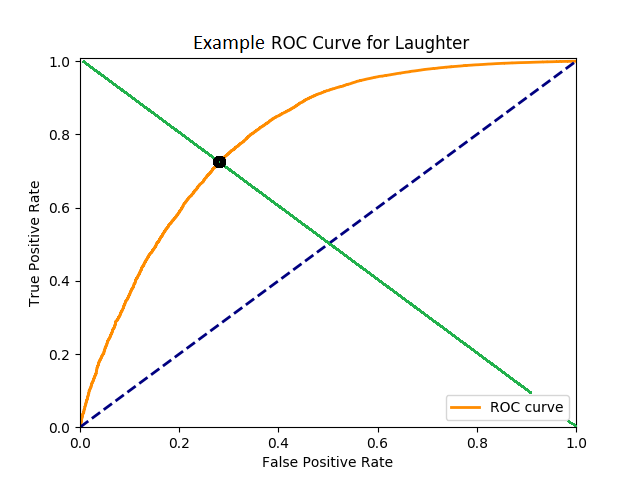
\includegraphics[scale = 0.7]{figs/laughter_roc.png}
	\caption{An ROC curve displaying the accuracy of a system when using different discrimination thresholds. A black dot has been placed on the point of equal error rate.}
	\label{laughter_roc1}
\end{figure}

\noindent
The most commonly used metric for evaluating systems for laughter detection is the `equal error rate' \cite{reuderink2008decision,kennedy2004laughter,truong2005automatic,knox2007automatic,petridis2008fusion}. This can be easily seen in ROC curves, and is the point on the ROC curve where the fraction of false positives is equal to the fraction of false negatives. This point is the equal error rate, and is aimed to be reduced. Visually, the point of equal error rate can be found quite easily if a line is drawn from the top left corner to the bottom right corner. The intersection of this line with the ROC curve is the point of equal error. 

\newpage
\section{Results}

% Talk about the metrics of the best network I made.
% Talk about the node features of the best network I made. (For each learning model)
% Talk about results from different networks
	% The single frame network
	% The multi frame network
% Best accuracy of different hyperparameter networks.

\newpage
\section{Discussion}

% Maybe the in depth results will take place in this section, and not above.
% Talk about funky things that my networks have picked up. All the weird things.
% Different features of the audio my system is picking up.

\subsection{Node Weights}
\subsection{Optimisation Algorithm}

\subsection{Improvements and Future Study}

% Talk about the myriad of features I'm sure I will have wished I could get around to, and would love to see the results of, but didn't quite have enough time to do.
% If someone else were to do this thesis, the things I would have liked them to do are:
	% Different types of laughs: genuine vs polite

\newpage
\section{Conclusion}

% Conclude. Another brief summary of everything I have done, and close.

\newpage

\bibliography{report}
\bibliographystyle{IEEEtran}

\end{document}
